\chapter{Diseño e Implementación}
\label{cap:capitulo4}

El objetivo de este \ac{TFG} es desarrollar un sistema de conducción autónoma capaz de realizar seguimiento de carril, control adaptativo al tráfico y maniobras de adelantamiento completas de manera segura en un entorno simulado y controlado. En este capítulo, se establecen primero los fundamentos de la percepción, definiendo qué elementos del entorno pueden ser detectados y qué información estará disponible para los modelos de control. A continuación, se implementa un sistema de conducción autónoma tradicional basado en el seguimiento de carril mediante un controlador \ac{PID}. Posteriormente, se exploran algunos algoritmos de \ac{DRL}) aplicados a la conducción autónoma, desarrollando y evaluando distintos modelos para la generación de comportamientos inteligentes. Finalmente, se lleva a cabo un análisis comparativo de los diferentes enfoques implementados, destacando sus ventajas e inconvenientes en el contexto de la conducción autónoma en un escenario de carreras.

\section{Arquitectura general}

El simulador CARLA nos proporciona un entorno de simulación avanzado que incluye el vehículo a controlar, la generación de tráfico, circuitos de prueba, así como sensores y actuadores simulados.

Entre los sensores disponibles contamos con cámaras y sensores \ac{LiDAR}, los cuales permiten obtener información detallada del entorno. Estos datos son procesados en el bloque de percepción, donde se aplican herramientas avanzadas de detección de carril y segmentación semántica sobre las imágenes capturadas, así como un tratamiento inteligente de los datos provenientes del \ac{LiDAR}. El objetivo de este procesamiento es extraer información relevante y simplificada, que servirá como observaciones para los modelos de conducción autónoma.

Los modelos de conducción autónoma, tanto los tradicionales como los basados en \ac{DRL}, procesan esta información para aprender a tomar decisiones óptimas y robustas en tiempo real. Estas decisiones se aplican directamente a los actuadores del vehículo dentro del simulador CARLA.

El comportamiento resultante de estos procesos, así como las relaciones entre los distintos bloques funcionales del sistema, pueden observarse reflejados en el diagrama de diseño \ref{fig:arch}.

\begin{figure}[ht]
  \centering
  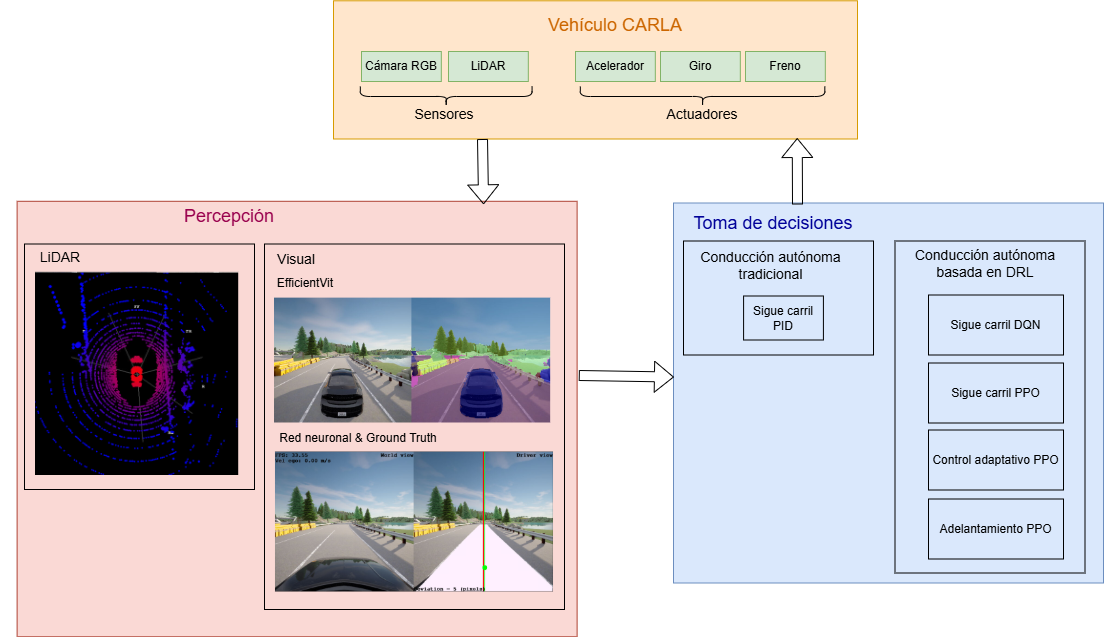
\includegraphics[width=16cm]{figs/Diseño/arquitectura.png}
  \caption{Arquitectura general.}
  \label{fig:arch}
\end{figure}

\section{Percepción visual}

La percepción visual se basa en las imágenes captadas por una cámara RGB, un sensor simulado en CARLA, con una resolución de 512 x 512 píxeles. Esta cámara se coloca con una perspectiva similar a la de un conductor. En esta sección, veremos cómo, a partir de esa información y aplicando diversas herramientas, es posible identificar el carril y segmentar la imagen.

\subsection{Detección de carril}

El objetivo es utilizar cada una de las herramientas de detección de carril para identificar los límites derecho e izquierdo del carril. Ademas, se definide una altura máxima para la detección del carril, creando así la forma de un trapecio. Al unir los puntos a la misma altura, podemos obtener el área del carril, su centro de masas y la desviación del coche con respecto al carril, considerando el centro de la imagen como el centro de nuestro vehículo.

\begin{code}[h]
\begin{lstlisting}[language=Python]

for i in range(limitis_for[0], limitis_for[1]): # Altura
	if not self._lane_network: # Ground truth
		x_left, y = self._lane_left[i]
		x_right, _ = self._lane_right[i]
	else: # Deteccion de carril DL
		y = i
		x_left = max(int(y * coef_left[0] + coef_left[1]), 0)
		x_right = min(int(y * coef_right[0] + coef_right[1]) + 1, SIZE_CAMERA - 1)

	if x_left < x_right:
		img[y, x_left:x_right] = (255, 240, 255)
\end{lstlisting}
\caption[Detección y cálculo de la superfice del carril]{Detección y cálculo de la superfice del carrill.}
\label{code:detectar_carril}
\end{code}

Teniendo los puntos límite del carril en todas las alturas, también es sencillo calcular \textit{n} puntos de cada línea del carril igualmente espaciados en el eje y. En la Figura \ref{fig:puntos_carril}, se muestra un ejemplo de cómo se obtienen diez puntos de cada línea del carril. Estos puntos, junto con el centro de masas, el área y la desviación del carril, constituyen una representación simplificada del carril para el modelo de conducción autónoma.

\begin{figure}[ht]
  \centering
  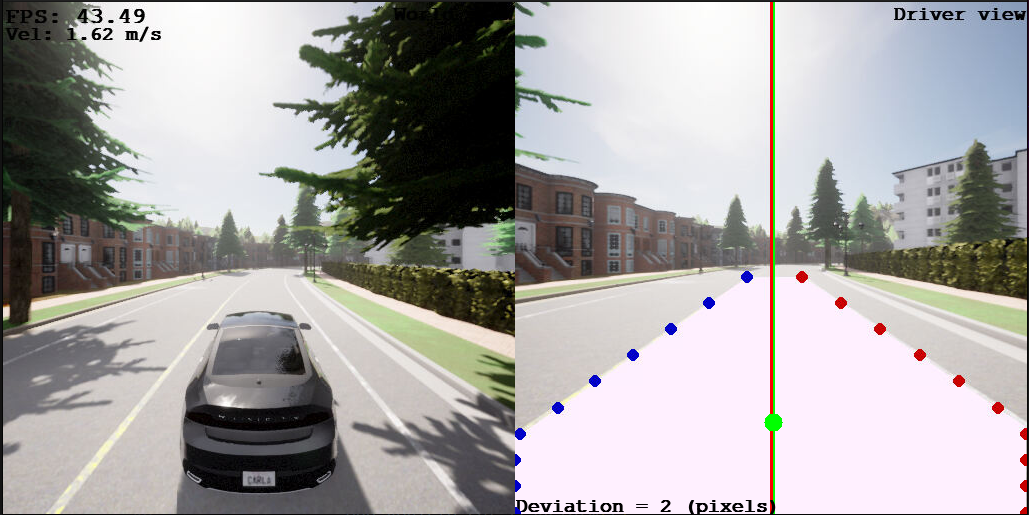
\includegraphics[width=11cm]{figs/Diseño/lane/lane10.png}
  \caption{Representación del carril: superficie, centro de masas, desviación y puntos de sus líneas.}
  \label{fig:puntos_carril}
\end{figure}

\subsubsection{Modelo basado en \ac{DL}}

El modelo de \ac{DL} para la detección de carril procesa imágenes de 512 x 1024 píxeles. Para ello, primero creamos una imagen vacía y colocamos la del carril en el centro. Esta imagen se pasa como entrada al modelo, el cual devuelve dos máscaras que definen las líneas del carril. Para mejorar la detección, especialmente en situaciones donde las líneas están discontinuas o cuando la red neuronal devuelve líneas fragmentadas o incompletas, aplicamos regresión lineal a los puntos obtenidos para cada línea. Este procedimiento nos permite calcular los coeficientes de las rectas que mejor se ajustan a esos puntos, y con ello, conocer sus límites.

\begin{figure}[ht]
  \centering
  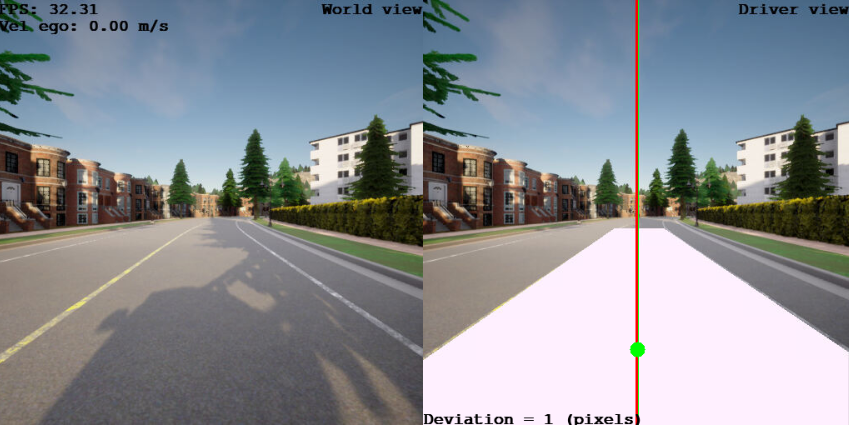
\includegraphics[width=10cm]{figs/Diseño/lane/red_neuronal_carril.png}
  \caption{Detección de carril basada en \ac{DL}.}
  \label{fig:dl_final_carril}
\end{figure}

A pesar de esta regresión, hemos implementado una técnica para eliminar los \textit{outliers} de cada máscara. Solo conservamos los puntos que caen dentro de un umbral determinado a partir de la medida anterior. En la Figura \ref{fig:outliers}, se ilustra este proceso utilizando la siguiente codificación de colores:

\begin{figure}[ht]
  \centering
  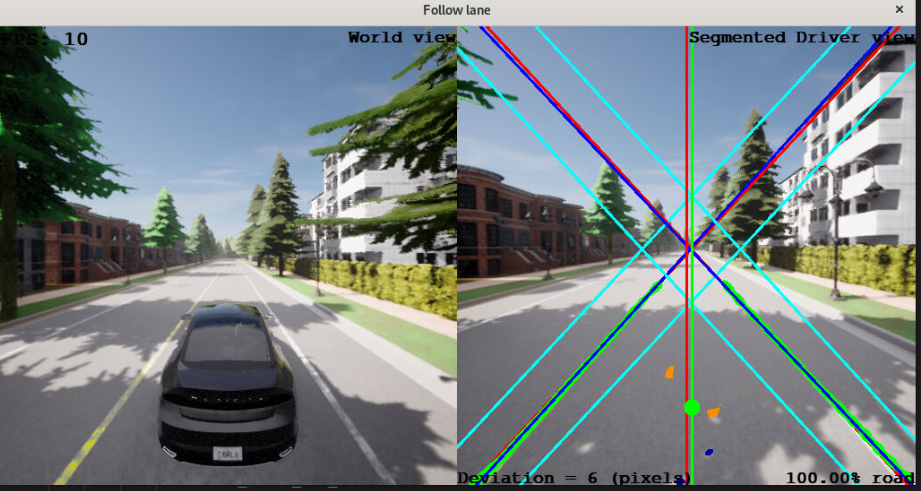
\includegraphics[width=11cm]{figs/Diseño/lane/remove_outliers.png}
  \caption{Eliminación de \textit{outliers} en la detección de carril basada en \ac{DL}.}
  \label{fig:outliers}
\end{figure}

\begin{itemize}
		\item Las líneas rojas en forma de cruz representan las dos detecciones de cada línea de carril previas.
		\item Las líneas cian que rodean a las anteriores delimitan la zona válida.
		\item Los puntos verdes son los puntos válidos que se tendrán en cuenta para la detección del carril, mientras que los puntos azules o naranjas representan los \textit{outliers}.
		\item Las líneas azules son el resultado de aplicar regresión lineal sobre los puntos válidos (verdes).
\end{itemize}

De esta manera, conseguimos una detección más precisa del carril. Además, se ha implementado un sistema de memoria para filtrar mediciones erróneas. Este sistema almacena las cinco últimas detecciones de las líneas, junto con el ángulo que cada una forma con la horizontal. Si el ángulo de la detección actual difiere lo suficiente de la media de los ángulos almacenados o si no se detecta ninguna línea, descartamos la medida y utilizamos la última detección válida. Si esto ocurre durante más de cinco iteraciones consecutivas, determinamos que se ha perdido el carril.

\begin{code}[h]
\begin{lstlisting}[language=Python]
index_mask = np.where(mask > self._threshold_lane_mask)
coefficients = np.polyfit(index_mask[0], index_mask[1], 1)

# Comprobar la medida
mean = np.mean(self._coefficients[:, index, 2])  
angle = math.degrees(math.atan(coefficients[0])) % 180  

if  abs(mean - angle) > MAX_ANGLE:
    self._count_mem_lane[index] += 1 
    return False  # Tomamos medida anterior
else:
    self._count_mem_lane[index] = 0  # Reiniciar contador memoria
    self._coefficients[-1, index, 0:2] = coefficients 
    self._coefficients[-1, index, 2] = angle

\end{lstlisting}
\caption[Detección de carril \ac{DL}: regresión lineal y validación de medida]{Detección de carril \ac{DL}: regresión lineal y validación de medida.}
\label{cod:dl_carril}
\end{code}

\subsubsection{Ground truth}

Una vez aplicado el \textit{ground thruth}, obtenemos algunos puntos del límites del carril, pero no todos. Para obtener los límites completos del carril, utilizamos la función \textit{pygame.draw.lines}. Sin embargo, esta función solo devuelve el rectángulo que rodea la línea dibujada, pero no los puntos de la línea en sí. Por lo tanto, dibujamos la línea sobre una superficie negra y luego analizamos esta superficie para localizar los límites del carril en términos de píxeles. Para optimizar el rendimiento computacional, restringimos la búsqueda al área dentro del rectángulo que encierra la línea. Al encontrar un punto, detenemos la búsqueda, ya que, dado que la línea es continua, podemos asumir con certeza que en cada altura habrá un punto que marcará el límite del carril. Si buscamos el límite izquierdo, comenzamos desde el inicio de la imagen (x = 0), mientras que, si buscamos el límite derecho, empezamos desde el final de la imagen. El siguiente código ilustra este proceso:
\begin{code}[h]
\begin{lstlisting}[language=Python]

rect = pygame.draw.lines(black_surface, (255, 0, 0), False, projected_boundary, 4)
pixels = []
for y in range(rect.top, rect.bottom):
    for x in range(start, end, step):
        color = black_surface.get_at((x, y))
        if color[0] == 255:
            pixels.append((x, y)) # Limites del carril
            break

\end{lstlisting}
\caption[Identificación de puntos del carril con información de \textit{ground thruth}]{Identificación de puntos del carril con información de \textit{ground thruth}.}
\label{cod:gt_carril}
\end{code}

\newpage

Como se mencionó en la sección anterior, este enfoque resulta más fiable que la detección de carril mediante \ac{DL}, ya que, a pesar de los posibles obstáculos que puedan afectar la visibilidad, es capaz de seguir detectando el carril gracias a la información obtenida directamente del simulador CARLA. Por lo tanto, esta será la técnica empleada durante los entrenamientos, ya que, en ciertos escenarios, es necesario tener un vehículo delante que pueda ocultar temporalmente las líneas del carril.

\begin{figure}[ht]
  \centering
  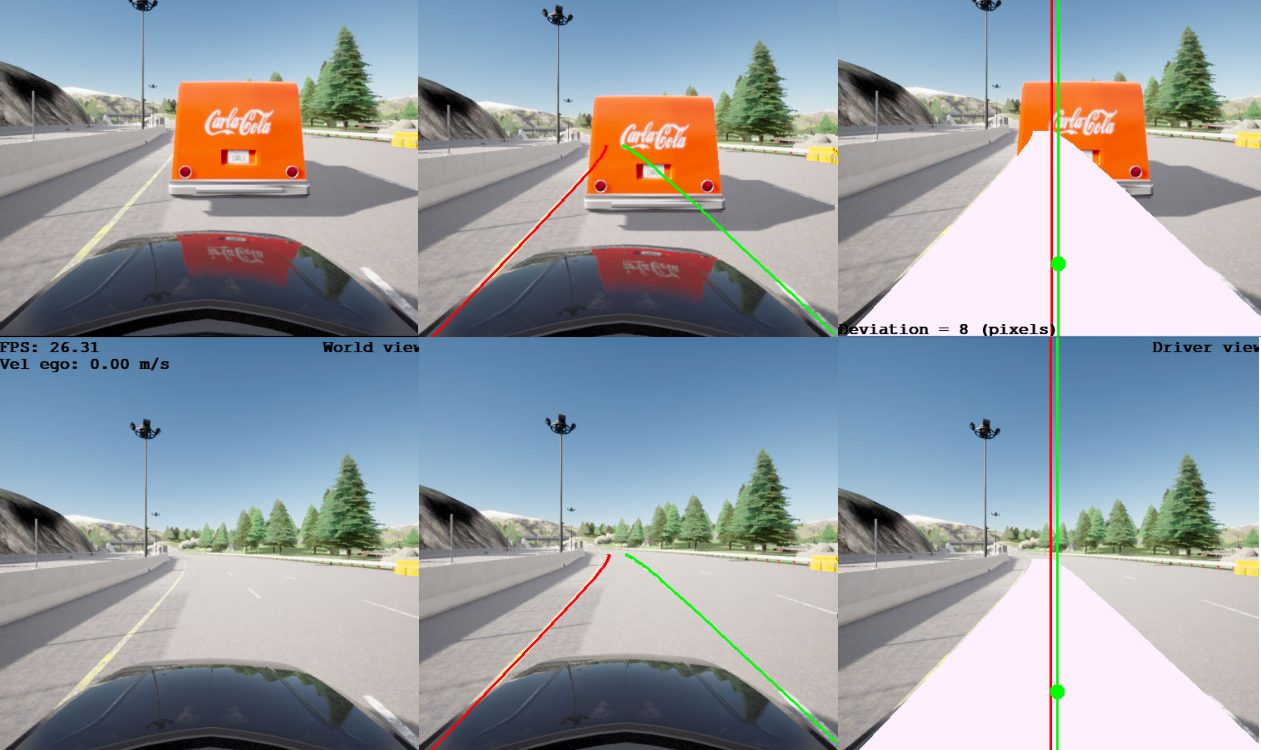
\includegraphics[width=11cm]{figs/Diseño/lane/ground_truth.png}
  \caption{Detección de carril basada en \textit{ground thruth}.}
  \label{fig:gt_final_carril}
\end{figure}

\subsection{Segmentación la calzada}

Con la red neuronal de segmentación semántica, podemos conocer con precisión los límites y área de la calzada. Al igual que para el carril, necesitamos una representación simplificada de la misma, para ello, analizamos la máscara de segmentación que nos proporciona EfficientVit para calcular su área, centro de masas y dieciséis puntos igualmente espaciados de cada límite lateral de la calzada. Con el fin proporcionar información más valiosa al modelo, seleccionamos solo un cuarto de los puntos de la parte totalmente vertical, como se puede apreciar en la Figura \ref{fig:seg_params}. Para implementar esta funcionalidad nos hemos apoyado principalmente en la librería NumPy.

\begin{figure}[ht]
  \centering
  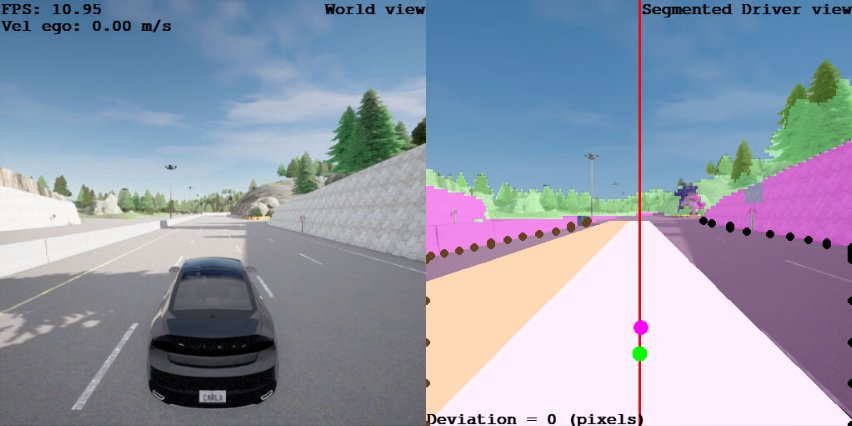
\includegraphics[width=10cm]{figs/Diseño/seg_points.png}
  \caption{Representación de la calzada: superficie, centro de masas y límites.}
  \label{fig:seg_params}
\end{figure}

También se utiliza la segmentación comprobar el porcentaje del área del carril que es carretera y para saber si hay un carril a la izquierda que nos permita llevar a cabo la maniobra de adelantamiento. Para hacer esta última comprobación, replicamos el carril actual a la izquierda y comprobamos que porcentaje de esta área es calzada, zona naranja en la Figura \ref{fig:seg_params}.

\section{Percepción con el \ac{LiDAR}}

El \ac{LiDAR} es un sensor simulado de CARLA que proporciona como salida una nube de puntos que indica la distancia y la posición de los objetos en el entorno, permitiendo una reconstrucción de la escena para la percepción y navegación del vehículo autónomo. Se configura el \ac{LiDAR} con un alcance máximo de 19.5 metros, distancia suficiente para detectar obstáculos en la carretera, en nuestro caso otros vehículos. Para la representación gráfica de la información del \ac{LiDAR}, mostramos cada uno de los puntos de la nube en 2D, coordenadas \textit{x} e \textit{y}. Con el fin de mejorar la percepción visual, se ha interpolado el color de cada punto según su intensidad, siendo tonos rojos los valores más altos y azules los más bajos, y el tamaño según su altura, a mayor elevación mayor tamaño.
\begin{figure}[ht]
  \centering
  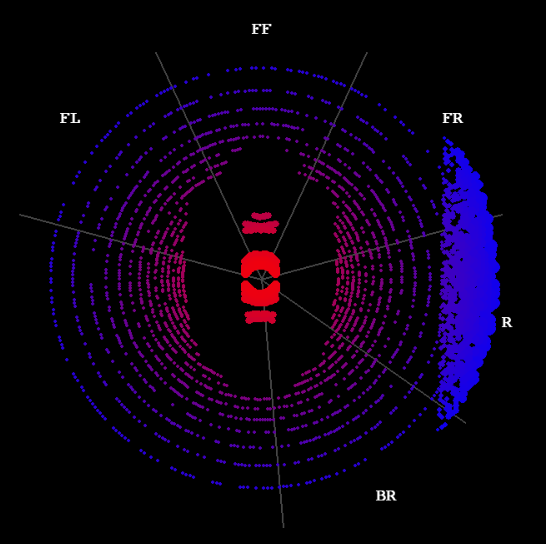
\includegraphics[width=7cm]{figs/Diseño/lidar/interpolate.png}
  \caption{Visualización de la nube de puntos generada por el \ac{LiDAR}.}
  \label{fig:interpolate_lidar}
\end{figure}

Con el fin de realizar un control adaptativo respecto al coche de delante, nos enfocamos en analizar la zona frontal del \ac{LiDAR} con una amplitud de 150º, dividida en tres subzonas de 50º: \textit{front-left}, \textit{front}, \textit{front-right}. Para determinar los ángulos que delimitan estas zonas independientemente de cómo se disponga el \ac{LiDAR} en el vehículo, debemos tener en cuenta la rotación del \ac{LiDAR} en el eje z (\textit{yaw}). Al ángulo deseado, la mitad de la zona frontal, le restamos el \textit{yaw} real y finalmente lo acotamos en un rango de [-180º, 180º]. Aunque ya hemos encontrado los ángulos extremos, es necesario calcular los dos ángulos intermedios que delimitan las tres zonas. Para ello, sumamos la amplitud de cada subzona al primer ángulo límite y se la restamos al segundo. En nuestro caso, con un \textit{yaw} de 90º, obtenemos los ángulos: [-165.0, -115.0, -65.0, -15.0]. 
\begin{code}[h]
\begin{lstlisting}[language=Python]
angle1 = get_angle_range(-self._front_angle / 2 - yaw)
angle2 = get_angle_range(self._front_angle / 2 - yaw)

angle1_add = get_angle_range(angle1 + self._front_angle / 3)
angle2_sub = get_angle_range(angle2 - self._front_angle / 3)        
self._angles = [angle1, angle1_add, angle2_sub, angle2]
\end{lstlisting}
\caption[Cálculo de los ángulos de la zona frontal del \ac{LiDAR}]{Cálculo de los ángulos de la zona frontal del \ac{LiDAR}.}
\label{cod:angle_lidar}
\end{code}

Como se puede observar en el dibujo \ref{fig:dib_angle}, dependiendo de que ángulo sea mayor, debemos seguir un criterio u otro para determinar si un punto pertenece o no la zona de interés o a una subzona concreta.
\begin{figure}[ht]
  \centering
  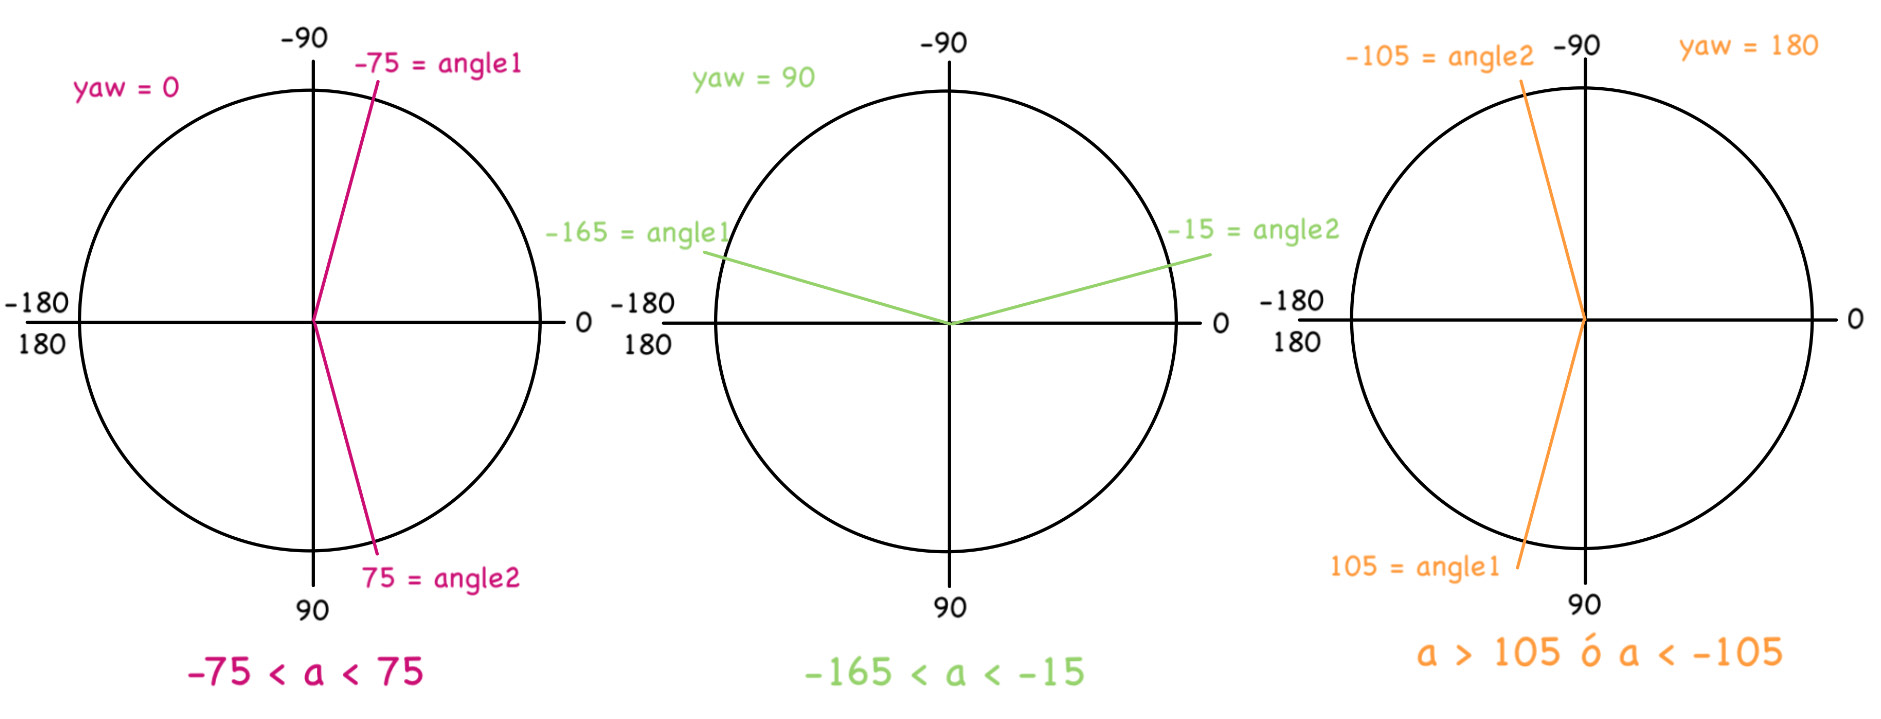
\includegraphics[width=10cm]{figs/Diseño/lidar/draw_angles.jpg}
  \caption{Criterio para saber a qué zona pertenece un punto del \ac{LiDAR}.}
  \label{fig:dib_angle}
\end{figure}

Para tener información adicional además de la visual, se ha creado un cálculo de estadísticas para cada subzona: mínimo, media, mediana y desviación estándar. Como se puede observar en la Figura \ref{fig:interpolate_lidar}, los puntos de color rojo corresponden al propio coche, por lo tanto, hemos realizado un filtrado por intensidad para eliminarlos de los cálculos estadísticos. De la misma manera, filtramos por altura para eliminar todos los puntos correspondientes a la calzada y otros elementos del entorno externos a la carretera (montañas, árboles…), quedándonos solo con información relevante para la conducción.
\begin{figure}[ht]
  \centering
  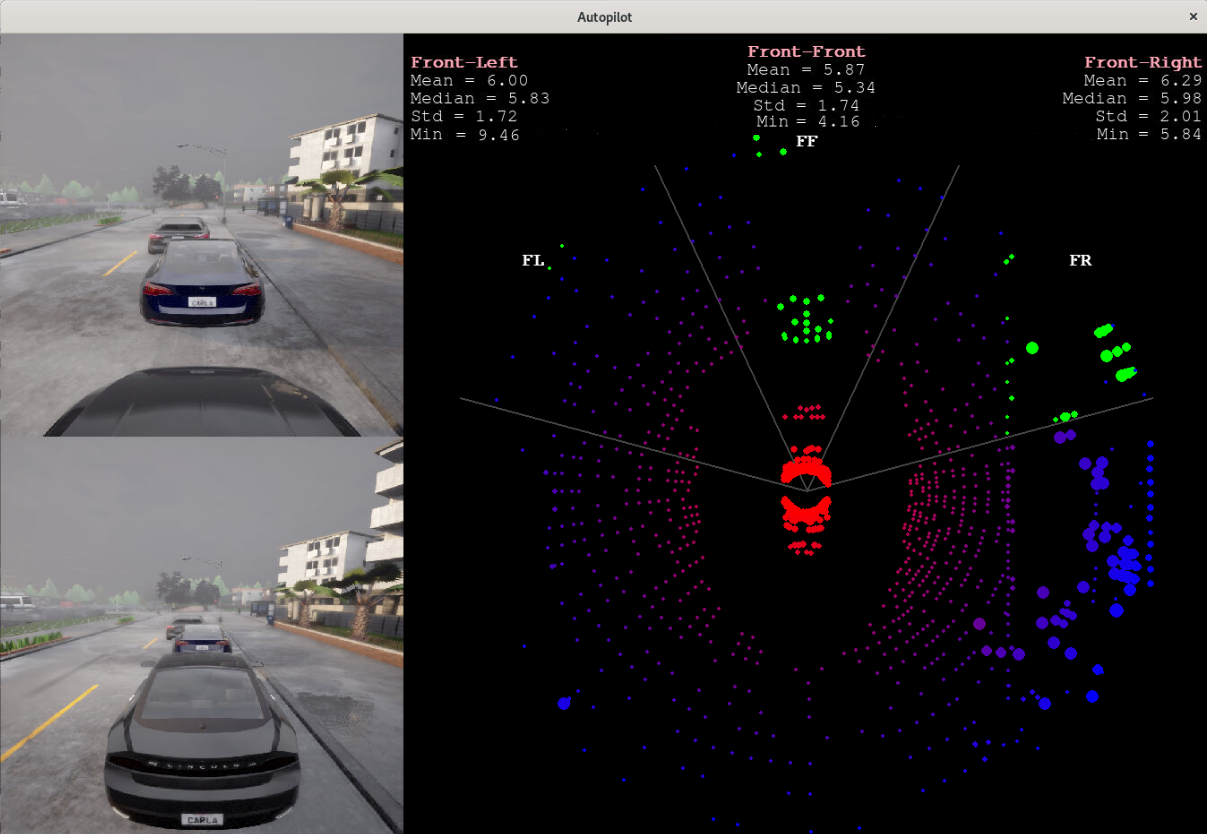
\includegraphics[width=10cm]{figs/Diseño/lidar/stats.png}
  \caption{Criterio para saber a qué zona pertenece un punto del \ac{LiDAR}.}
  \label{fig:dib_angle}
\end{figure}

Para saber cuándo poder volver al carril durante un adelantamiento, se han añadido dos subzonas en la parte derecha del \ac{LiDAR}: \textit{right} y \textit{back-right}. De nuevo, para intentar tener en cuenta solo información que concierne a la conducción, se ha realizado un filtrado por distancia dependiendo de la subzona, ya que, por ejemplo, necesitamos más rango del en la zona frontal del \ac{LiDAR} que en la lateral. De esta manera, nos aseguramos que el modelo recibe solo puntos dentro de la carreta. Los filtros de distancia aplicados según la zona son los siguientes:
    \begin{itemize}
        \item \textit{Front}: no aplicamos filtro distancia, disponemos del rango máximo del \ac{LiDAR}.
        \item \textit{Right-front}: nos quedamos con distancias iguales o menores a 7m.
        \item \textit{Right}: filtrado por distancia de 6m.
        \item \textit{Right-back}: filtramos distancias inferiores a 9m.
    \end{itemize}

Una vez aplicados todos los filtros descritos, se ha implementado una función que extrae un número determinado de puntos de cada subzona, ordenados y equiespaciados en el eje \textit{x} , para ser utilizados como observaciones en los modelos.
\begin{figure}[ht]
  \centering
  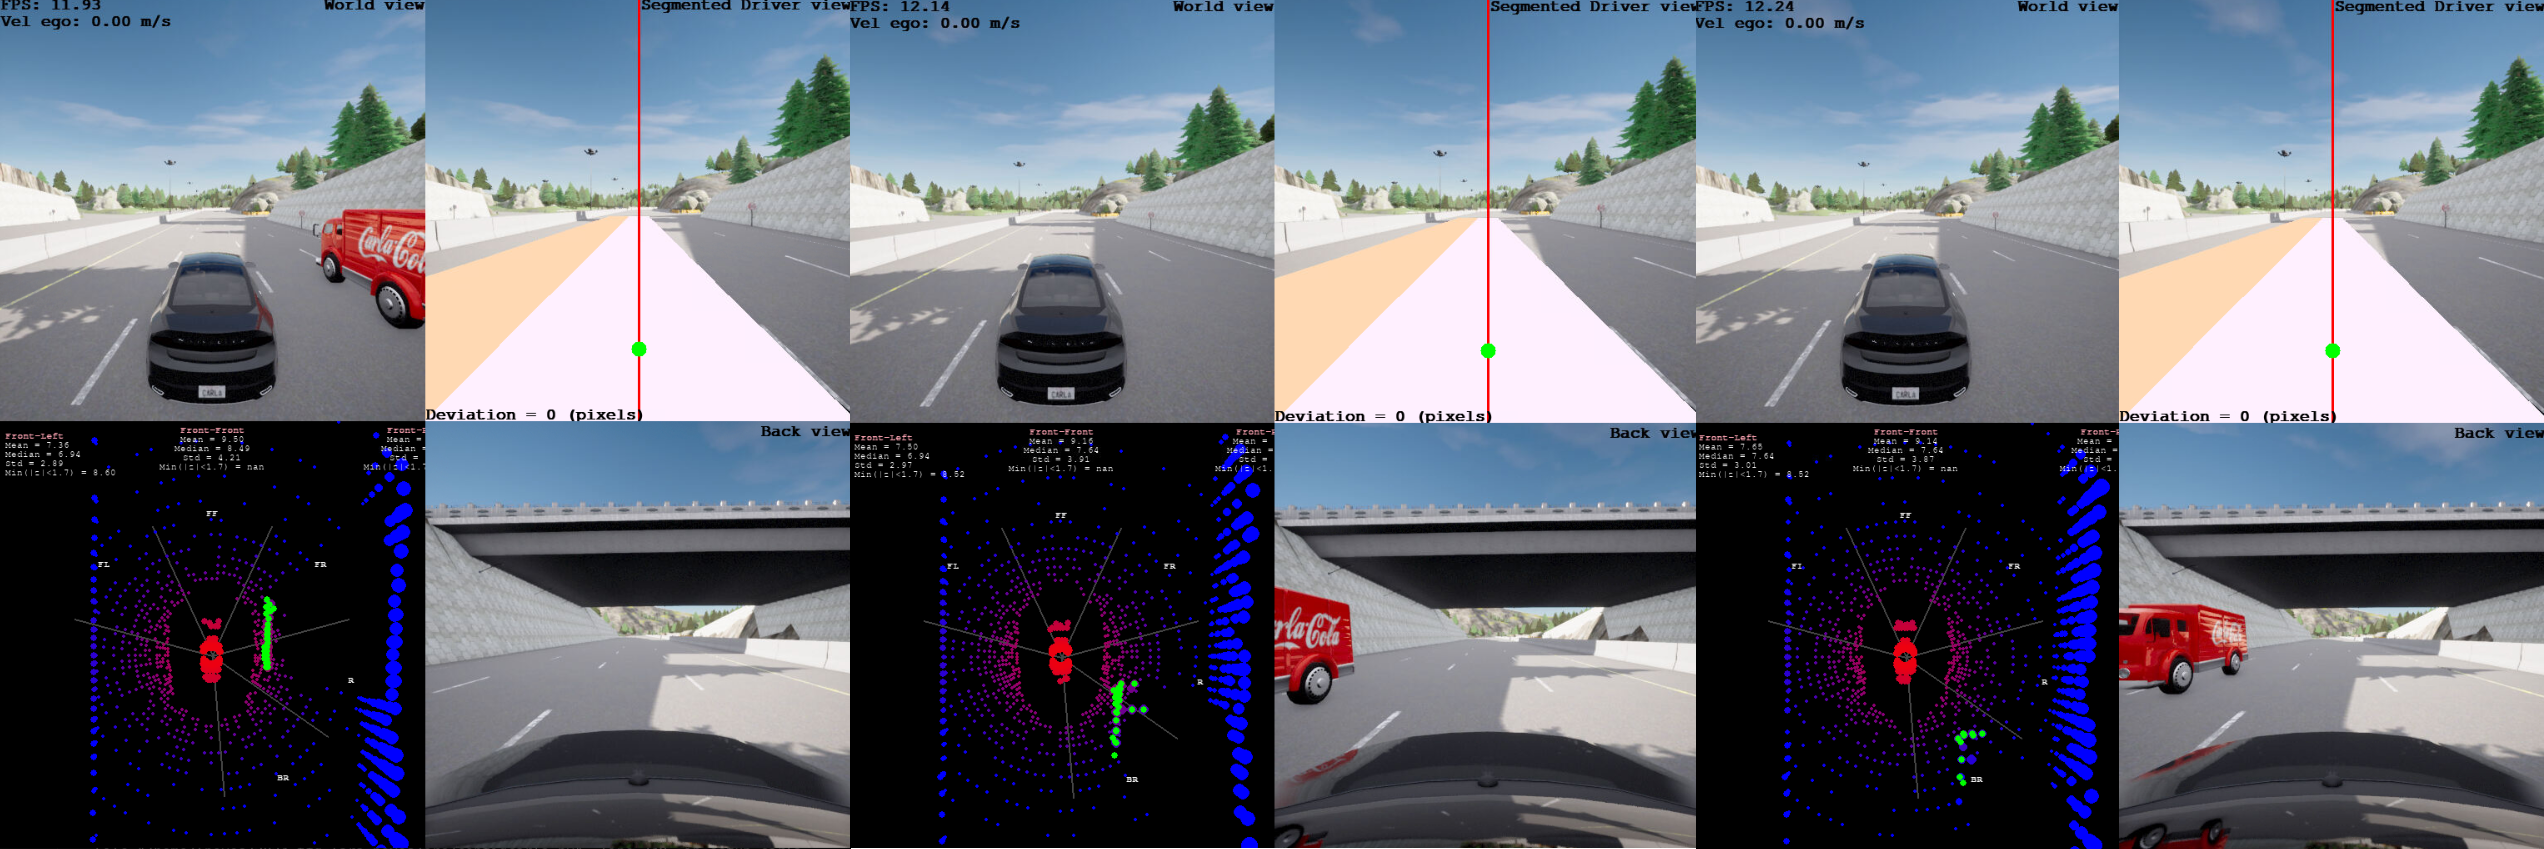
\includegraphics[width=11cm]{figs/Diseño/lidar/laser_right.png}
  \caption{Filtrado del \ac{LiDAR} zona derecha.}
  \label{fig:laser_right}
\end{figure}

\begin{figure}[ht]
  \centering
  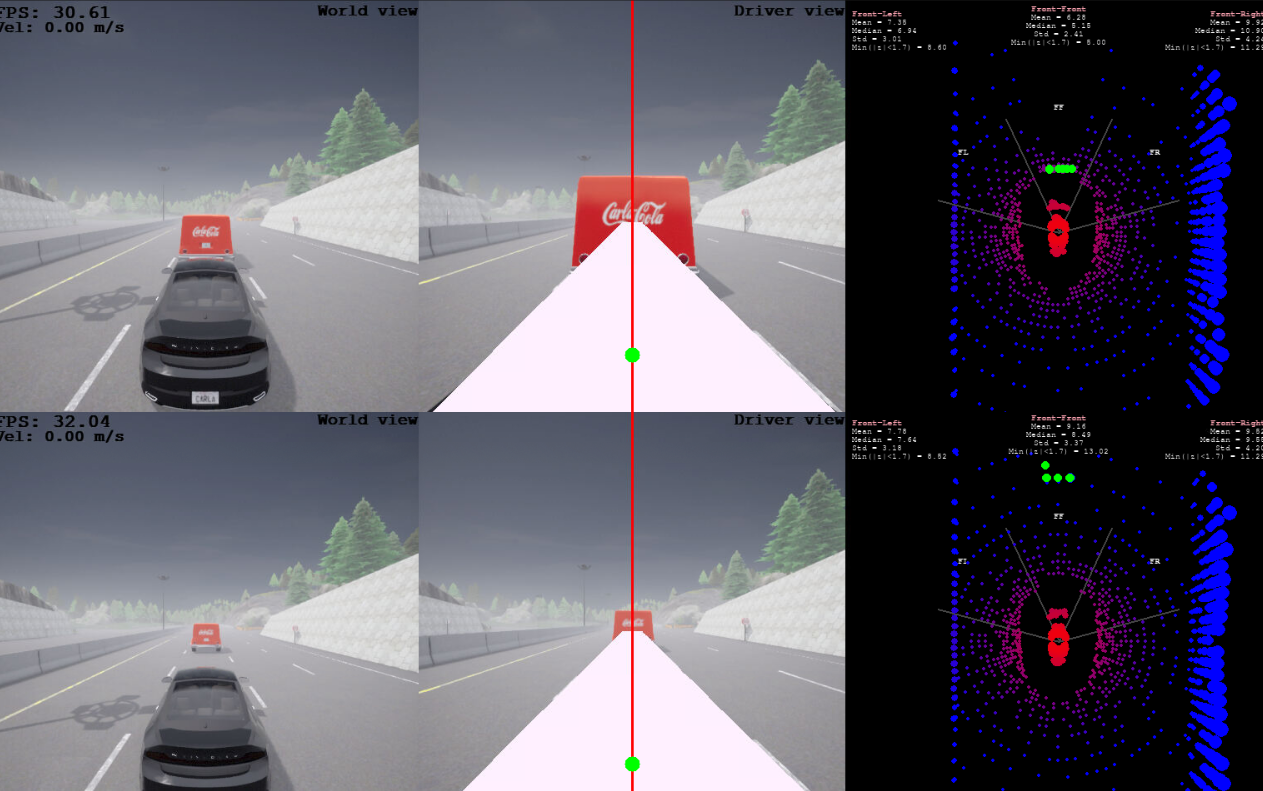
\includegraphics[width=11cm]{figs/Diseño/lidar/laser_front.png}
  \caption{Filtrado del \ac{LiDAR} subzona frontal.}
  \label{fig:laser_front}
\end{figure}

Se llevó a cabo un \textit{profiling} para evaluar las latencias y determinar dónde estamos consumiendo más tiempo en nuestrocódigo, con el objetivo de mejorar su eficiencia. Como se puede observar en la Figura \ref{fig:profiling}, la mayor parte del tiempo se destina a realizar la predicción con EfficientVit. El resto de secciones presentan latencias acordes a su carga computacional, sin presenta una desventaja significativa en proceso de entrenamiento e inferencia.
\begin{figure}[ht]
  \centering
  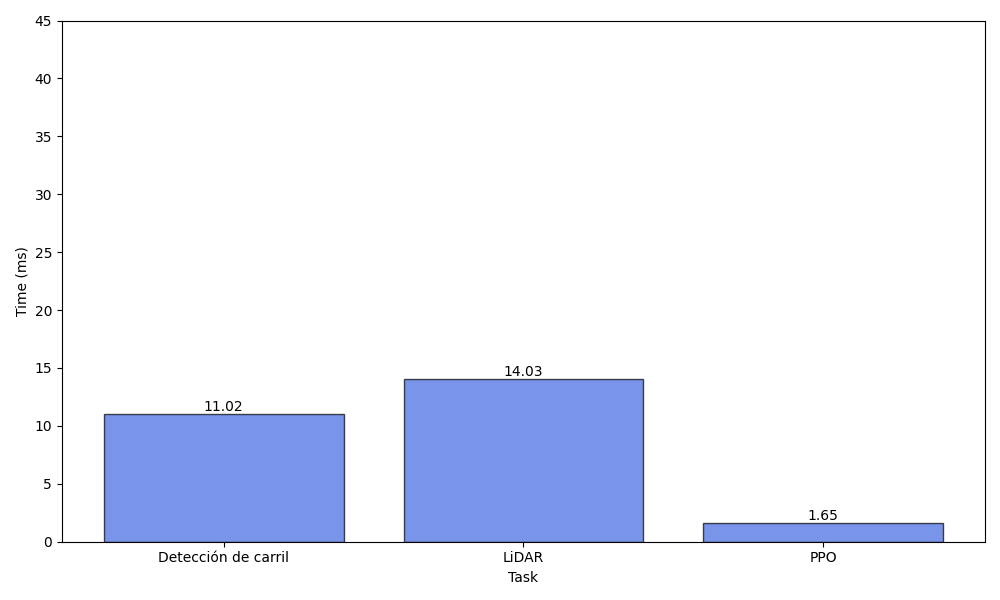
\includegraphics[width=16cm]{figs/Diseño/profiling.png}
  \caption{\textit{Profiling} del proceso percepción.}
  \label{fig:profiling}
\end{figure}

\section{Conducción autónoma tradiconal}

El proceso de toma de decisiones en la conducción autónoma tradicional está a basado en reglas predefinidas y sistemas matemáticos, sin aprovechar las capacidades del \ac{ML}, lo que limita su adaptación a entornos dinámicos y situaciones imprevistas. Para este tipo de conducción, se requieren modelos matemáticos complejos y muy detallados del vehículo y del entorno si desea un desempeño preciso y seguro. Una toma de decisiones tan rígida basada en reglas fijas y algoritmos deterministas no es adecua para situaciones reales donde la incertidumbre en un factor clave, necesitamos modelos capaces de adaptarse a escenarios cambiantes. 

A pesar de ello, existen técnicas de control clásico que funcionan adecuadamente para ciertas habilidades de conducción. Un controlador \ac{PID} es un tipo de control ampliamente utilizado en sistemas automáticos para ajustar una variable y mantenerla en un valor deseado. En conducción autónoma, se usa para mantener un vehículo en el carril ajustando el ángulo del volante según la desviación del carril.

\subsection{Controlador \ac{PID} para el seguimiento de carril}
Para el seguimiento de carril basado en un controlador tradicional \footnote{\url{https://youtu.be/mq5STc8-Z6Y}}, se ha implementado un controlador PD para controlar el giro. Al mismo tiempo, el acelerador se mantiene fijo a 0.5, mientras que con el freno regula la velocidad para mantenerla constante a aproximadamente 10m/s.
\begin{code}[h]
\begin{lstlisting}[language=Python]
self._kp = 1 / (SIZE_CAMERA / 2)
self._kd = -self._kp / 1.7
self._throttle = 0.5
\end{lstlisting}
\caption[Definición de contantes para el controlador \ac{PID}]{Definición de contantes para el controlador \ac{PID}.}
\label{cod:const_pid}
\end{code}

En la parte de percepción, ya hemos calculado la desviación respecto al centro del carril del vehículo. Esta desviación representa el error que recibe nuestro controlador. El componente proporcional se encarga de normalizar el error en un rango compatible con CARLA [0.0, 1.0], mientras que el signo del error ya indica el sentido del giro. Si el error supera cierto umbral, lo incrementamos ligeramente para mejorar el rendimiento en las curvas. El componente derivativo evita movimientos oscilatorios al salir de las curvas, ya que resta el error anterior reducido. Este componente resta el valor del error anterior, pero solo lo consideramos si su signo es diferente al del error actual, ya que, de lo contrario, podría causar inestabilidad y afectar negativamente la conducción durante las curvas.
\begin{code}[h]
\begin{lstlisting}[language=Python]
# Difrente signo
if (self._error > 0 and self._prev_error < 0) or (self._error < 0 and self._prev_error > 0):
	self._prev_error = 0       

# Aumento del error
if error > 20:
	error *= 1.15

control.steer = self._kp * error + self._kd * self._prev_error
\end{lstlisting}
\caption[Regulación del giro mediante el controlador \ac{PID}]{Regulación del giro mediante el controlador \ac{PID}.}
\label{cod:pid_giro}
\end{code}

\section{Conducción autónoma basada en \ac{DRL}}

Como vimos en la primera sección, el aprendizaje por refuerzo utiliza una \textit{Q-table} para encontrar las acciones que proporcionaban mayor recompensa, pero esto ya no es una forma práctica de modelar la función de transición de estado-acción, especialmente cuando el espacio de estados es muy extenso o continuo, tendríamos que explorar cada estado al menos una vez para encontrar la mejor solución. En su lugar, los algoritmos de \ac{DRL} utilizan una \textit{Q-network}, red neuronal diseñada para aprender la función que mapea estados-acciones. Esta red es capaz de estimar el valor de estados no explorados, ya que aprende las relaciones entre los diferentes pares estado-acción. En una \textit{Q-table}, los valores se almacenan en una tabla, mientras que en una \textit{Q-network} se guarda en los pesos de la red. Esta red recibe los estados del entorno como entrada y produce como salida el valor de cada acción posible. 

El \ac{DRL} es un enfoque en el que los agentes de aprendizaje por refuerzo utilizan redes neuronales para tomar decisiones. Esta combinación les permite adaptarse mejor a entornos complejos donde las reglas no son evidentes ni fácilmente definibles, como es el caso de la conducción autónoma. Dentro de los algoritmos de \ac{DRL}, existen dos tipos claramente diferenciados:

\begin{itemize}
		\item \textit{On-policy:} Son aquellos que actualizan el modelo solo con datos de la política actual, una vez que la política cambia, los datos anteriores se vuelven inservibles y se descartan.
		\item \textit{Off-policy:} Son aquellos que pueden usar cualquier dato recolectado durante el entrenamiento, independientemente de la política con la que hayan sido obtenidos.

\end{itemize}

En este \ac{TFG}, solo se han utilizado los algoritmos de \ac{DQN} y \ac{PPO}, los cuales son \textit{off-policy} y \textit{on-policy} respectivamente\cite{drl}.

\subsection{Seguimiento de carril con \ac{DQN}}

\ac{DQN} es un algoritmo de \ac{DRL} que soportar un espacio de estados complejo y continuo, pero el espacio de acciones es discreto. Las acciones en un espacio discreto son predefinidas y limitadas, es decir, no existe una continuidad entre ellas, sino que están representadas por un número finito de opciones que el agente puede elegir en cada estado.

\ac{DQN} es un algoritmo \textit{off-policy} ya que incluye una \textit{replay memory}. Esta técnica consiste en crear una memoria de reproducción de experiencias que almacena las k experiencias más recientes que un agente ha recopilado, ya que son las más relevantes, para así poder reutilizarlas. Si la memoria está llena, se descarta la experiencia más antigua para dar espacio a la más reciente. En cada paso de entrenamiento, se muestrea uno o más lotes de datos de forma aleatoria de la memoria para actualizar los parámetros de la red. El tamaño de la memoria debe ser lo suficientemente grande como para contener experiencias de diferentes episodios y políticas, lo que ayuda estabilizar y mejorar el entrenamiento. Al actualizar en cada paso del entrenamiento la red neuronal, la minimización del error entre las predicciones de la red y los valores reales se vuelve complicada. Para abordar este problema, se introduce una nueva red neural, \textit{target networ}, diseñada para aportar estabilidad al proceso de entrenamiento. La nueva red es una réplica de la red principal, \textit{policy network}, pero en lugar de actualizarla en cada paso, la igualamos a la red original cada cierto número de pasos, manteniendo un objetivo de entrenamiento constante \cite{drl}.

Ahora que ya sabemos en qué consiste el algoritmo de \ac{DQN}, llega la hora de construir el entorno de entrenamiento para que un coche autónomo sea capaz de seguir el carril. Primero, debemos elegir el circuito de entrenamiento para nuestro modelo, para ello, hemos elegido el Town04 de CARLA, ya que incluye tramos largos y sin intersecciones. Como vemos en la Figura \ref{fig:mapa}, se han definido cuatro rutas, las rutas uno, dos y tres se utilizan durante el entrenamiento, mientras que la cuatro se usa para examinar el modelo en inferencia y comprobar si es capaz de generalizar. Cada una de estas rutas de entrenamiento comienza en una dirección distinta: curva a la derecha, línea recta y curva a la izquierda, con el fin de evitar \textit{overfitting} en el modelo.

\begin{figure}[ht]
  \centering
  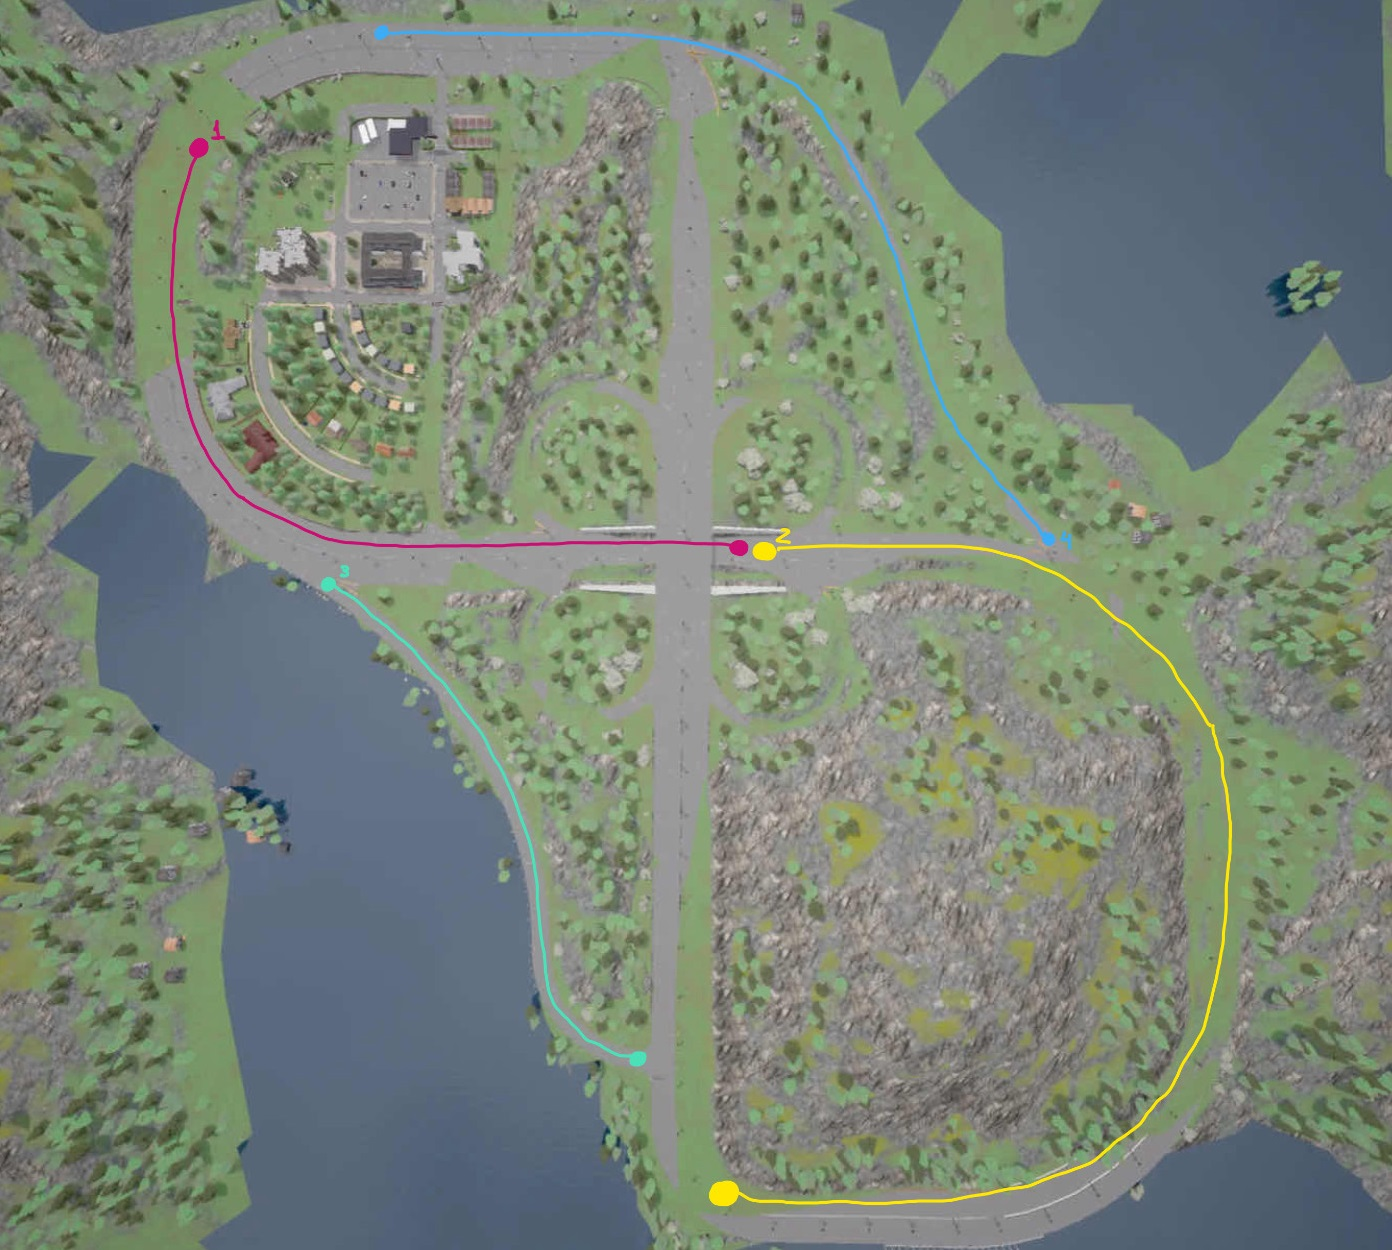
\includegraphics[width=10cm]{figs/Diseño/mapa.jpeg}
  \caption{Mapa del entorno de entrenamiento en CARLA con rutas definidas.}
  \label{fig:mapa}
\end{figure}

\newpage

El vehículo autónomo incorpora los sensores:
\begin{itemize}
		\item Cámara RGB: se utiliza para la detección de carril. Si se pierde la percepción, sale el carril o cambia de carril se genera una excepción que se captura y finaliza el episodio.
		\item Sensor de colisión: si el coche se choca contra un elemento del entorno también detenemos el episodio.
\end{itemize}

El espacio de observaciones coincide con el espacio de estados y está basado en un diccionario, por lo tanto, empleamos la política \textit{MultiInputPolicy}. Las observaciones se normalizan para facilitar el aprendizaje al modelo e incluyen la siguiente información: 
\begin{itemize}
		\item Desviación del carril.
		\item Área del carril.
		\item Cinco puntos de la línea izquierda del carril.
		\item Cinco puntos de la línea derecha del carril.
		\item Centro de masas.
\end{itemize}

\begin{figure}[ht]
  \centering
  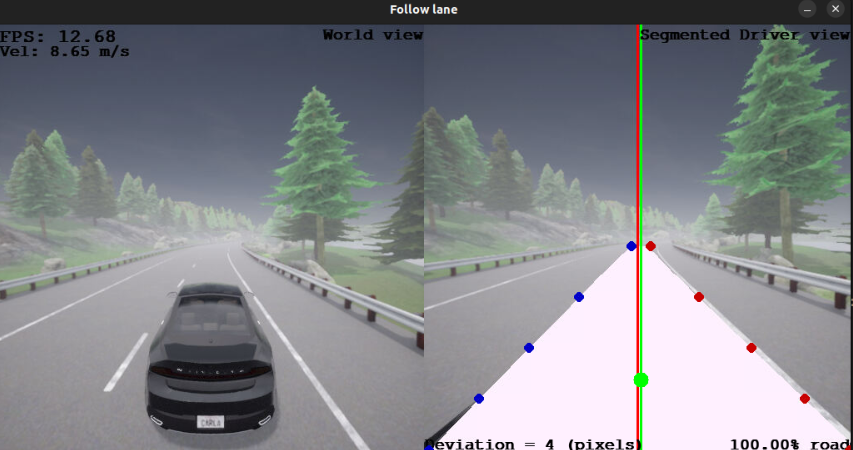
\includegraphics[width=9cm]{figs/Diseño/discrete/obs_dqn.png}
  \caption{Observaciones seguimiento de carril basado en \ac{DQN}.}
  \label{fig:dqn_obs}
\end{figure}

\newpage

Como hemos mencionado al inicio, \ac{DQN} permite un espacio de acciones discreto. Las acciones están compuestas por un comando de acelerador y otro de giro, para combinarlo hemos seguido la regla de que, a mayor aceleración, menor es el giro. En total, se han definido 21 acciones disponibles entre las cuales el coche autónomo podrá seleccionar aquellas que maximicen la recompensa en cada situación.

\begin{code}[h]
\begin{lstlisting}[language=Python]

self.action_to_control = {
    0: (0.5, 0.0),
    1: (0.45, 0.01), 
    2: (0.45, -0.01),
    3: (0.4, 0.02),
    4: (0.4, -0.02),
    5: (0.4, 0.04),
    6: (0.4, -0.04),
    7: (0.4, 0.06),
    8: (0.4, -0.06),
    9: (0.4, 0.08),
    10: (0.4, -0.08),
    11: (0.3, 0.1),
    12: (0.3, -0.1),
    13: (0.3, 0.12),
    14: (0.3, -0.12),
    15: (0.2, 0.14),
    16: (0.2, -0.14),
    17: (0.2, 0.16),
    18: (0.2, -0.16),
    19: (0.1, 0.18),
    20: (0.1, -0.18)
}
\end{lstlisting}
\caption[Acciones disponibles para el seguimiento de carril basado en \ac{DQN}]{Acciones disponibles para el seguimiento de carril basado en \ac{DQN}.}
\label{cod:acc_dqn}
\end{code}

Nuestro objetivo es que el coche circule por el centro del carril sin desviarse, manteniendo una conducción fluida y lo más rápida posible. Para lograrlo, hemos diseñado una función de recompensa que se basa principalmente en la desviación del carril y en la velocidad actual del coche, normalizando y ponderando estos valores según sus respectivos pesos. Sin embargo, si el coche pierde el carril o colisiona, el episodio se detiene y se asigna una recompensa negativa.

\begin{code}[h]
\begin{lstlisting}[language=Python]
if error == None:
      # Clip deviation and velocity
      r_dev = (MAX_DEV - abs(np.clip(self._dev, -MAX_DEV, MAX_DEV))) / MAX_DEV
      r_vel = np.clip(self._velocity, 0.0, self._max_vel) / self._max_vel
      reward = 0.8 * r_dev + 0.2 * r_vel
else:
      reward = -30
\end{lstlisting}
\caption[Función de recompensa sigue-carril basado en \ac{DQN}]{Función de recompensa sigue-carril basado en \ac{DQN}.}
\label{cod:rew_dqn}
\end{code}

Para entrenar el modelo hemos utilizado un \textit{fixed\_delta\_seconds} de 50ms, lo que equivale a entrenar a 20 \ac{FPS}, por lo tanto, en infrencia necesitamos operar al menos a esta velocidad. Los entrenamientos tuvieron una duración de un día y un par de horas. Tras realizar diversas pruebas experimentales, identificamos los hiperparámetros de entrenamiento que proporcionan los mejores resultados. 
\begin{code}[h]
\begin{lstlisting}[language=yaml]
learning_rate: 0.0005 # Tasa de aprendizaje
buffer_size: 20_000 # Capacidad de la memoria
batch_size: 1024 # Capacidad del lote
gamma: 0.85 # Factor de descuento: importancia de las recompensas futuras frente a las inmediatas
target_update_interval: 1024 # Intervalo de actualizacion de la red neuronal objetivo
train_freq: 256 # Frecuencia de entrenamiento
gradient_steps: 2 # Pasos de gradiente en cada actualizacion
exploration_fraction: 0.8 # Fraccion de exploracion
exploration_final_eps: 0.0 # Valor final de exploracion
n_timesteps: 8_000_000 # Numero total de steps

\end{lstlisting}
\caption[Hiperparámetros de entrenamiento para el sigue-carril basado en \ac{DQN}]{Hiperparámetros de entrenamiento para el sigue-carril basado en \ac{DQN}.}
\label{cod:hiper_params_dqn}
\end{code}

La frecuencia de entrenamiento resultó ser un factor clave en el proceso, al principio se utilizó un valor menor, pero los modelos no lograban converger. El ratio de exploración se reduce gradualmente durante el 80\% del entrenamiento y, a partir de ese punto, se dejan de realizar acciones aleatorias. En la siguiente gráfica, se puede observar cómo el modelo finalmente converge.
\begin{figure}[ht]
  \centering
  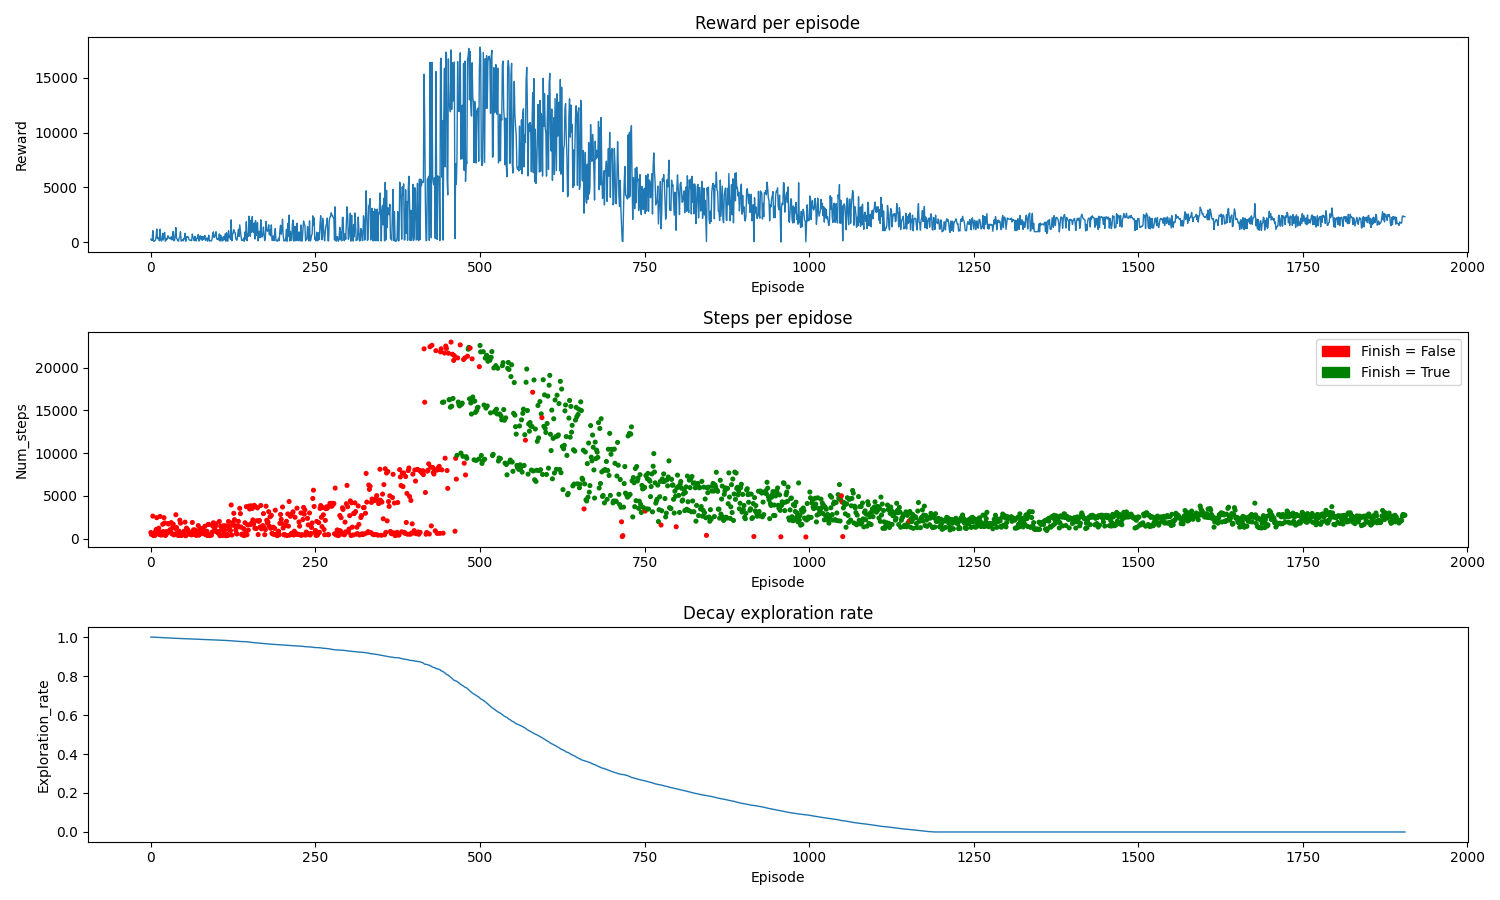
\includegraphics[width=13cm]{figs/Diseño/discrete/train_dqn.png}
  \caption{Gráfica de entrenamiento sigue-carril basado en \ac{DQN}.}
  \label{fig:train_dqn}
\end{figure}

\newpage

En inferencia en un circuito visto durante el entrenamiento \footnote{\url{https://youtu.be/rzy2Vg57zA8}}, se observa que el seguimiento del carril es bastante preciso, no obstante, ocasiones, se percibe un pequeño balanceo. Esto se debe a una de las limitaciones de \ac{DQN}, su espacio de acciones es discreto no permite seleccionar la acción de giro óptima en cada momento. A continuación, se presenta la información recopilada durante la inferencia. Podemos observar claramente los momentos en los que se reduce la velocidad, correspondientes a las dos curvas pronunciadas al inicio del circuito. Sin embargo, de forma general, los histogramas indican se eligen los pares de acciones más rápidos, llegando a alcanzar una velocidad de 14m/s.
\begin{figure}[ht]
  \centering
  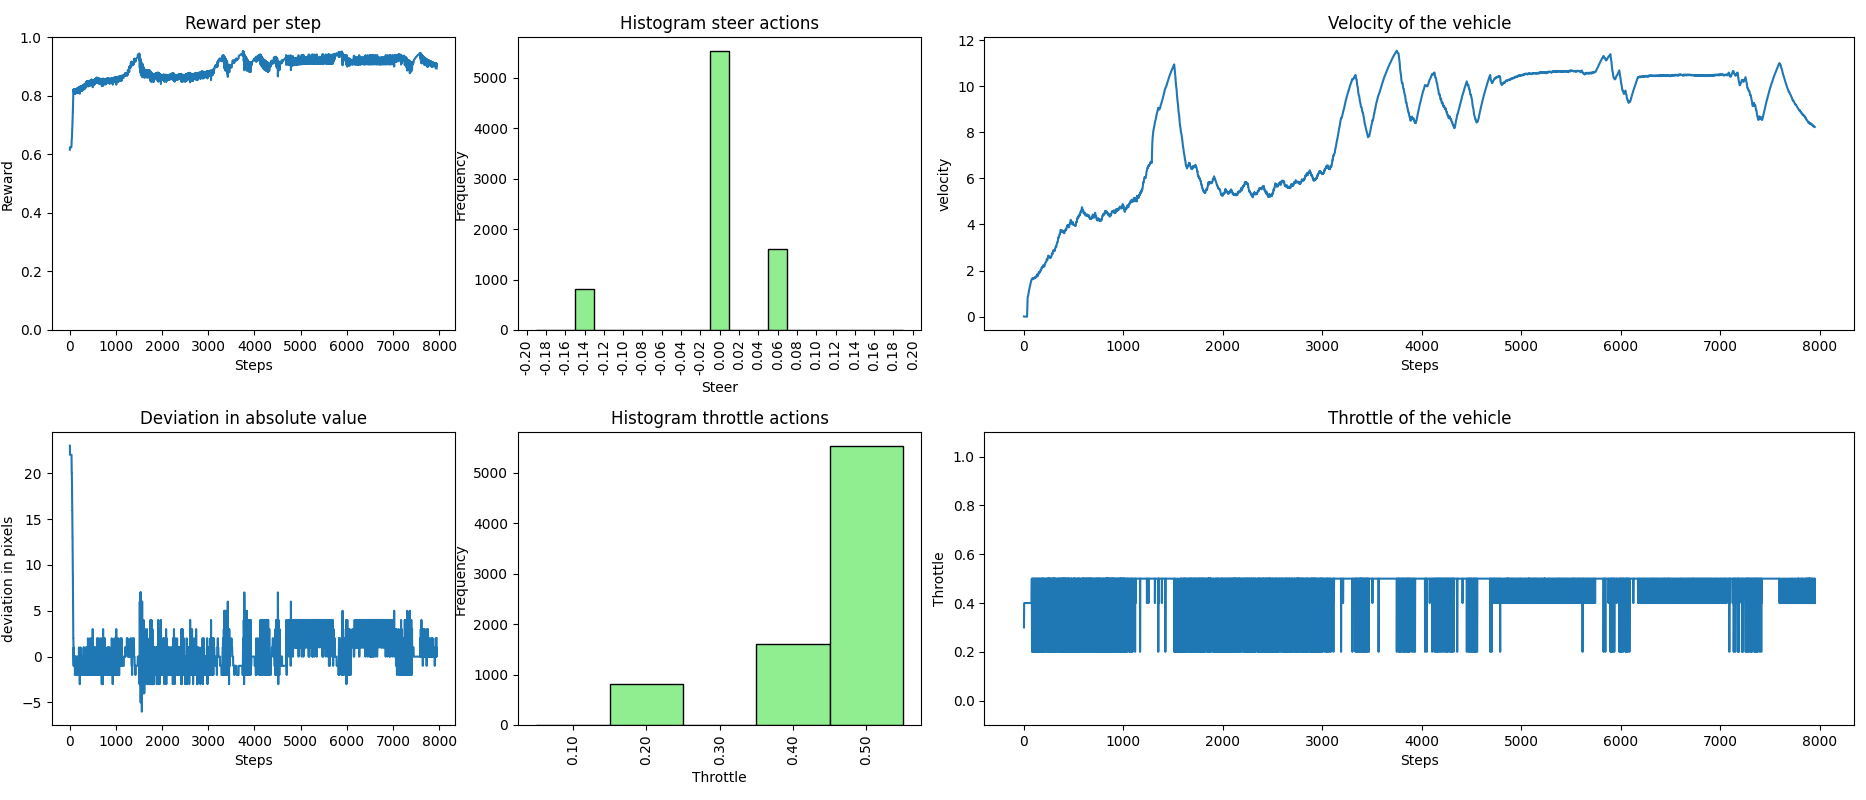
\includegraphics[width=15cm]{figs/Diseño/discrete/inference_dqn.png}
  \caption{Gráficas de inferencia sigue-carril basado en \ac{DQN}.}
  \label{fig:inference_dqn}
\end{figure}

\subsection{Seguimiento de carril con \ac{PPO}}

El algoritmo \textit{Actor-Critic} es un tipo de algortimo en el que cada agente consta de dos elementos que aprenden de manera conjunta, cada uno con su propia red neuronal: \textit{actor}, encargado de aprender la política óptima, y \textit{critic}, responsable de aprender la función de valor y proporcionar una señal de refuerzo a la política. El algoritmo \ac{A2C} se forma a partir de la unión del actor y el critic y es una algoritmo \textit{on-policy}. \ac{PPO} es un algoritmo \textit{on-policy} que puede considerarse como una extensión de \ac{A2C}, cuyo objetivo principal es evitar el deterioro del rendimiento. En los algoritmos basados en políticas, ajustar la tasa de aprendizaje puede ser una labor complicada. Un valor pequeño puede llevar a entrenamientos prolongados sin alcanzar la solución óptima, mientras que uno grande puede causar un colapso en el rendimiento. Con el objetivo de resolver esto, \ac{PPO} introduce un objetivo sustituto que asegura una mejora monótona del rendimiento, evitando cambios drásticos y arriesgados en la política que puedan afectar negativamente al despeño. Para lograrlo, \ac{PPO} mide cuánto ha cambiado la política después de cada actualización, garantizando que esta diferencia sea no negativa en cada iteración, asegurando así una mejora continua en el rendimiento. Además, que impide que esta razón crezca o disminuya demasiado dentro de un umbral controlado por un hiperparámetro (\textit{clip\_range}) \cite{drl}. 

El objetivo sigue siendo conseguir un seguimiento de carril fluido y la mayor velocidad posible, pero esta vez usamos el algoritmo \ac{PPO} que permite un espacio de acciones continuo. Se emplea la misma lógica para la finalización de un episodio, sensores, \textit{fixed\_delta\_seconds} de 50ms y circuito de entrenamiento \ref{fig:mapa} que en el entorno anterior. Seguimos controlando dos elementos: el acelerador y el giro, permitimos el rango completo para el acelerador y limitamos el rango del giro.

\begin{code}[h]
\begin{lstlisting}[language=Python]
self._max_steer = 0.2
self.action_space = spaces.Box(
    low=np.array([0.0, -self._max_steer]),
    high=np.array([1.0, self._max_steer]),
    shape=(2,),
    dtype=np.float64
)
\end{lstlisting}
\caption[Espacio de acciones sigue-carril basado en \ac{PPO}]{Espacio de acciones sigue-carril basado en \ac{PPO}.}
\label{cod:acc_ppo}
\end{code}

Sin embargo, se han llevado a cabo algunos cambios en las observaciones. Se ha añadido la velocidad actual del vehículo al espacio de observaciones para mejorar la comprensión de la función de recompensa y, en lugar de cinco, ahora el modelo recibe diez puntos de cada línea del carril, como se muestra en la Figura \ref{fig:puntos_carril}, para mejorar la comprensión del mismo, sobre todo en las curvas.

En este caso, la función recompensa es más compleja y sigue el siguiente esquema:
\begin{enumerate}
    \item \textit{Comprobación de errores:} Primero se verifica si ha ocurrido un error, como pérdida del carril o choque contra elementos de la carretera. Si ocurre, se finaliza el episodio y se asigna una recompensa negativa.

    \item \textit{Normalización lineal de elementos:} Si no hay errores, se normalizan los elementos de los que depende la recompensa:
    \begin{itemize}
        \item \textit{Desviación:} Se limita el valor de la desviación al rango [-100, 100]. Se normaliza inversamente, donde una desviación de 0 tiene la mayor recompensa.
        \item \textit{Giro:} Para giros bruscos, la recompensa es nula. Para giros no bruscos, se normaliza inversamente considerando el rango [-0.14, 0.14], donde menores giros otorgan mayor recompensa.
        \item \textit{Acelerador:} Si las aceleraciones son bruscas en el rango [0.6, 1.0], la recompensa es nula. Para aceleraciones no bruscas en el rango [0.0, 0.6), si se supera la velocidad máxima, se normaliza inversamente, aceleración nula tiene mayor recompensa. En el caso contrario, se normaliza de forma que mayores aceleraciones otorgan mayor recompensa.
    \end{itemize}

    \item \textit{Asignación de pesos a los elementos:} Finalmente, se define el peso de cada elemento en la recompensa según los siguientes criterios:
    \begin{itemize}
        \item Si el giro o el acelerador son bruscos, tienen un peso muy elevado en la recompensa, mientras que los otros dos elementos tienen un peso mucho menor.
        \item Si se supera la velocidad máxima, el acelerador tiene mayor peso para intentar decelerar, penalizando también el giro debido a la alta velocidad, puesto que puede tener un gran impacto.
        \item Si el acelerador es bajo, en el rango [0.0, 0.5), se penalizan menos los giros grandes, facilitando las curvas al reducir la velocidad.
        \item Si el acelerador está en un rango alto [0.5, 0.6), se penalizan más los giros bruscos, enfocándose en zonas rectas o con giros leves.
    \end{itemize}
\end{enumerate}

\begin{code}[H]
\begin{lstlisting}[language=Python]
if error is None:
    # Deviation normalization
    r_dev = (MAX_DEV - abs(np.clip(self._dev, -MAX_DEV, MAX_DEV))) / MAX_DEV

    # Steer conversion
    limit_steer = 0.14
    if abs(self._steer) > limit_steer:
        r_steer = 0
    else:
        r_steer = (limit_steer - abs(self._steer)) / limit_steer

    # Throttle conversion
    limit_throttle = 0.6
    if self._throttle >= limit_throttle:
        r_throttle = 0
    elif self._velocity > self._max_vel:
        r_throttle = (limit_throttle - self._throttle) / limit_throttle
    else:
        r_throttle = self._throttle / limit_throttle

    # Set weight
    if r_steer == 0:
        w_dev, w_throttle, w_steer = 0.1, 0.1, 0.8
    elif r_throttle == 0:
        w_dev, w_throttle, w_steer = 0.1, 0.8, 0.1
    elif self._velocity > self._max_vel:
        w_dev, w_throttle, w_steer = 0.1, 0.65, 0.25
    elif self._throttle < 0.5:
        w_dev, w_throttle, w_steer = 0.65, 0.25, 0.1
    else:  # Throttle in range [0.5, 0.6)
        w_dev, w_throttle, w_steer = 0.6, 0.15, 0.25

    reward = w_dev * r_dev + w_throttle * r_throttle + w_steer * r_steer
else:
    reward = -40
\end{lstlisting}
\caption[Función de recompensa para sigue-carril basado en \ac{PPO}]{Función de recompensa para sigue-carril basado en \ac{PPO}.}
\label{cod:rew_ppo}
\end{code}

Al igual que en el entrenamiento anterior, el hiperparámetro \textit{n\_steps} fue clave a la hora de adquirir convergencia, también influyó el tamaño del lote, que inicialmente era demasiado pequeño. Con valores bajos del coeficiente de entropía, el agente aprendía siempre que las acciones límite maximizaban la recompensa, mientras que, con valores demasiado altos, no conseguía converger. Finalmente, estos fueron los hiperparámetros de entrenamiento utilizados:
\begin{code}[h]
\begin{lstlisting}[language=yaml]
policy: "MultiInputPolicy"
learning_rate: 0.0001
gamma: 0.85
gae_lambda: 0.9
n_steps: 512 # Numero de pasos a ejecutar antes de cada actualizacion
batch_size: 512 
ent_coef: 0.1 # Coeficiente de entropia
clip_range: 0.15 
n_timesteps: 4_000_000
\end{lstlisting}
\caption[Hiperparámetros de entrenamiento para el sigue-carril basado en \ac{PPO}]{Hiperparámetros de entrenamiento para el sigue-carril basado en \ac{PPO}.}
\label{cod:hiper_params_ppo}
\end{code}

\newpage

Al analizar los parámetros de entrenamiento de ambos algoritmos, podemos ver como con \ac{PPO} necesitamos la mitad de \textit{steps} que con \ac{DQN} para lograr un entrenamiento exitoso. Los entrenamientos con \ac{PPO} duraron aproximadamente unas veinte horas. En el siguiente gráfico, se muestran los datos de entrenamiento, donde se puede observar cómo se logra rápidamente la convergencia, pero se necesitan más \textit{steps} para alcanzar altas velocidades.
\begin{figure}[ht]
  \centering
  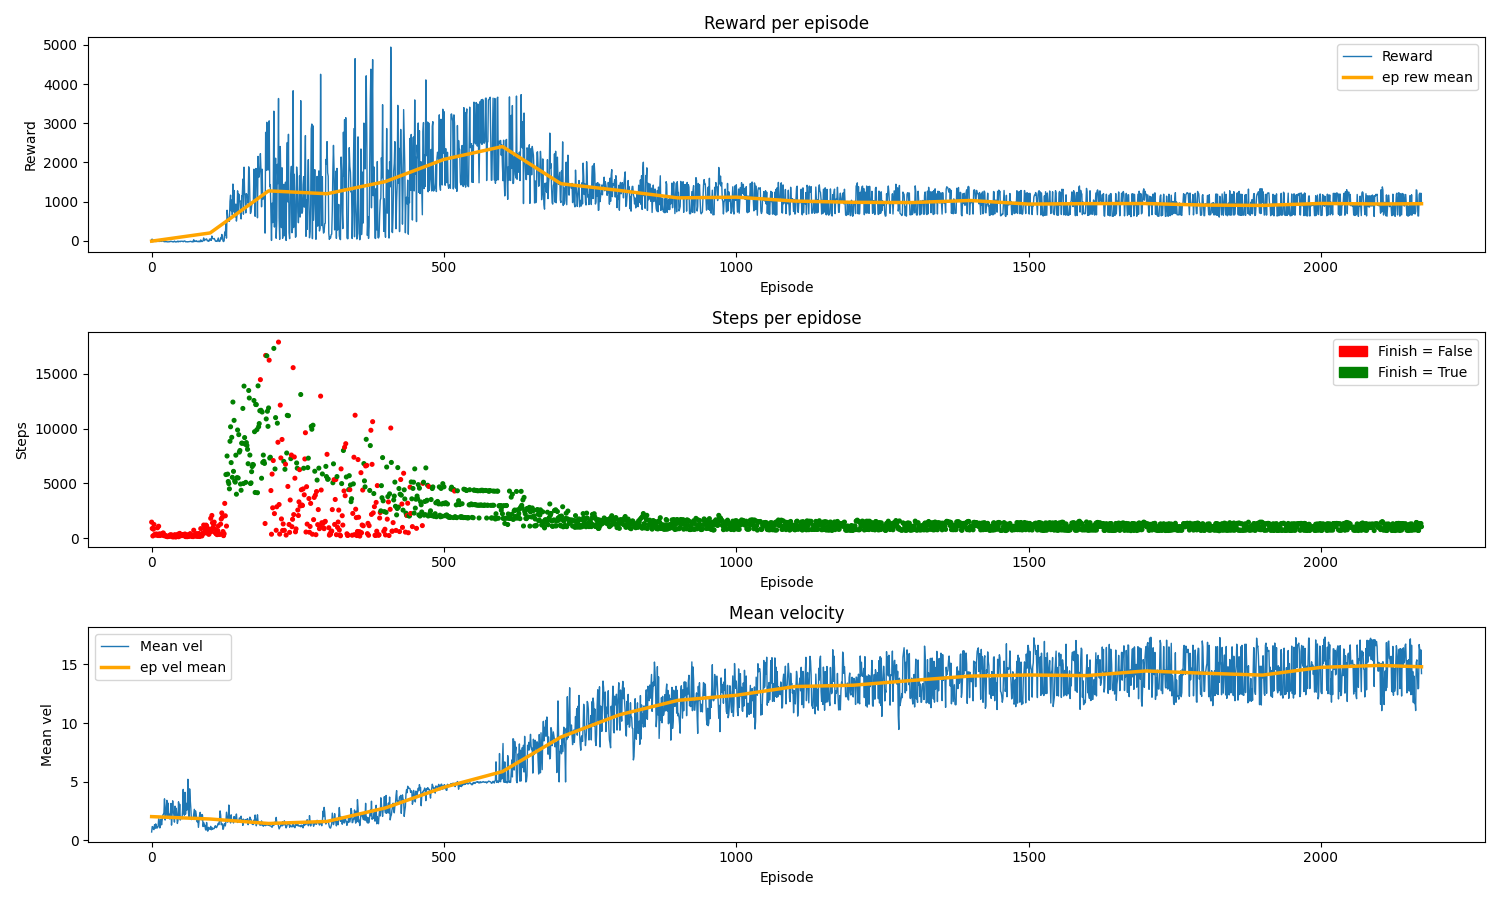
\includegraphics[width=13cm]{figs/Diseño/cont/train_ppo_carril.png}
  \caption{Gráficas de entrenamiento sigue-carril basado en \ac{PPO}.}
  \label{fig:train_ppo_carril}
\end{figure}

Debido a todos los inconvenientes con el coeficiente de entropía en  la exploración de acciones, también se desarrolló un programa para analizar la las frecuencia de las acciones tomadas durante el entrenamiento, cuyos resultados se presentan en el siguiente histograma.
\begin{figure}[ht]
  \centering
  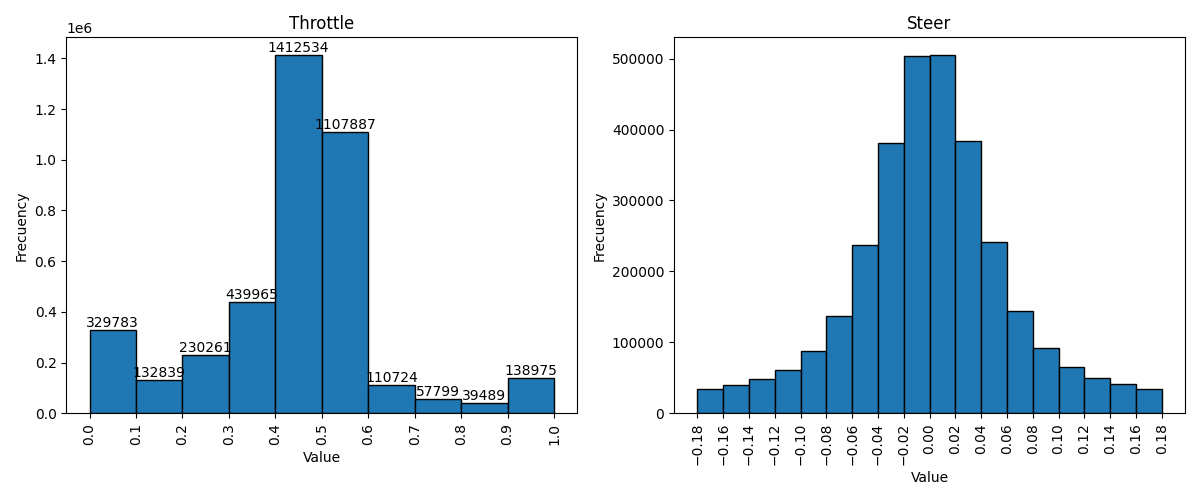
\includegraphics[width=11cm]{figs/Diseño/cont/actions_ppo_carril.png}
  \caption{Histogramas de acciones tomadas durante el entrenamiento sigue-carril basado en \ac{PPO}.}
  \label{fig:actions_ppo_carril}
\end{figure}

\newpage

En inferencia obtenemos muy buenos resultados tanto en circuitos utilizados durante el entrenamiento \footnote{\url{https://youtu.be/bZNfUwP14gc}} como en nuevos \footnote{\url{https://youtu.be/WRPLzKqJdto}}, incluso cambiando la ciudad en el simulador CARLA. A diferencia del modelo entrenado con \ac{DQN}, ahora si podemos elegir el giro exacto necesario en cada momento al disponer de un espacio de acciones continuo, lo que permite seguir el carril de forma más precisa y fluida. Además, se logran velocidades muy superiores, incluso superando los 20m/s. El modelo elige siempre aceleraciones en el rango [0.5, 0.6) combinadas con giros sutiles. Cabe destacar que, si eliminamos la parte del rango bajo del acelerador en la función recompensa, unificando ambos rangos en uno con los mismos pesos, el entrenamiento no logra converger, aunque al final siempre seleccione acciones en dentro del rango alto del acelerador.
\begin{figure}[ht]
  \centering
  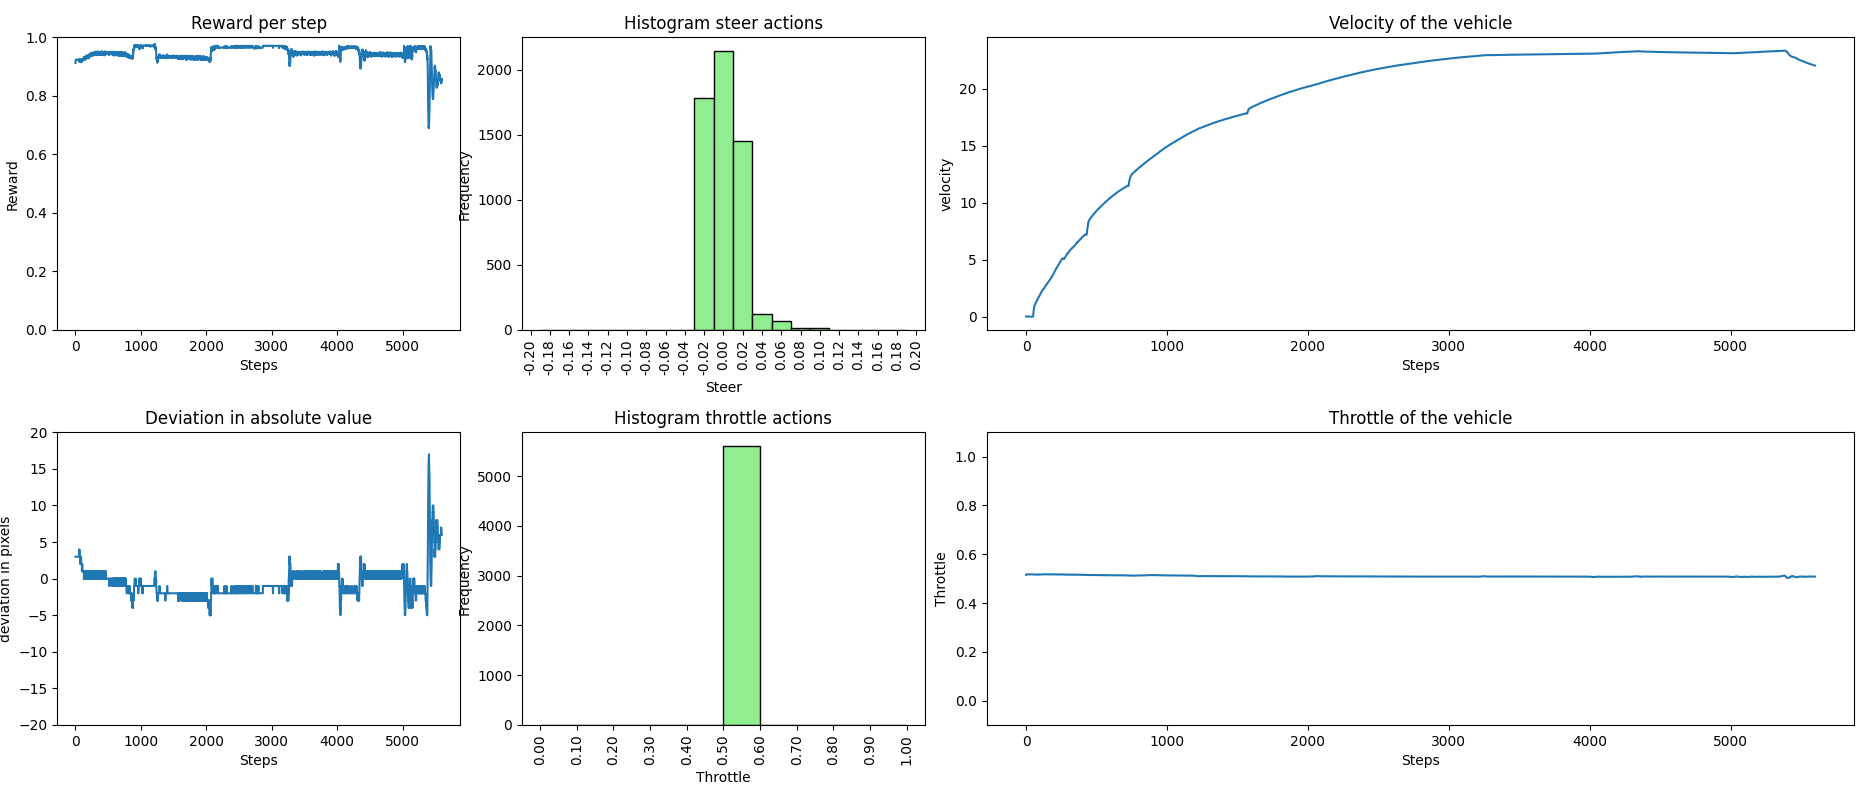
\includegraphics[width=15cm]{figs/Diseño/cont/inference.png}
  \caption{Gráfico de los datos recopilados durante inferencia del modelo sigue-carril con \ac{PPO}.}
  \label{fig:inference_ppo_carril}
\end{figure}

Recordemos, que los entrenamientos se han realizado utilizando la técnica de detección de carril \textit{ground thruth}. Si la cambiamos por la detección de carril basada en \ac{DL}, lo que incluye cambiar la posición de la cámara y, por tanto, la visión de percepción, seguimos obteniendo un seguimiento del carril fluido y conciso \footnote{\url{ https://youtu.be/8kOpXYqzIGM}} a altas velocidades.

\subsection{Control adaptativo con PPO}

Ahora el objetivo ha cambiado, el vehículo autónomo debe ser capaz de regular su velocidad en función del vehículo que tiene delante, controlado por el autopiloto de CARLA, además de seguir el carril. Para esta nueva funcionalidad, necesitamos añadir un nuevo sensor, el \ac{LiDAR}, cuyas observaciones son veinte puntos de la subzona frontal, como se muestra en la Figura \ref{fig:laser_front}. Mantenemos las mismas rutas de entrenamiento y resto de observaciones que en el apartado anterior. Seguimos utilizando el algoritmo de \ac{PPO} con el mismo espacio de acciones, ya que permite un control más fluido, preciso y un comportamiento más adaptativo al entorno. 

\begin{code}[h]
\begin{lstlisting}[language=Python]
self._num_points_laser = 20
self.observation_space[KEY_LASER] = spaces.Box(
	low=MIN_DIST_LASER - 1.0,
	high=MAX_DIST_LASER,
	shape=(self._num_points_laser,),
	dtype=np.float64
)
\end{lstlisting}
\caption[Definición de observación frontal del \ac{LiDAR}]{Definición de observación frontal del \ac{LiDAR}.}
\label{cod:obs_laser_front}
\end{code}

Un cambio clave respecto al modelo anterior es que, esta vez, hemos entrenado a 10 \ac{FPS} en lugar de 20 \ac{FPS}. A 20 \ac{FPS}, el agente no lograba un comportamiento adaptativo eficiente, sino un efecto de \textit{muelle}, acercándose demasiado al coche de delante, frenando bruscamente, alejándose y repitiendo el ciclo. En cambio, a 10 \ac{FPS}, se ha conseguido un comportamiento adaptativo más estable. Esto puede deberse a una reducción de ruido en las observaciones, los cambios en entorno y, por tanto, en las observaciones pueden ser más sutiles entre \textit{steps} consecutivos, permitiendo un mejor aprendizaje y compresión del escenario.

Para facilitar el aprendizaje del modelo, primero se realizado un entrenamiento exclusivamente para aprender a seguir el carril. Durante este entrenamiento, se ha \textit{congelado} la observación referente al \ac{LiDAR}, es decir, los puntos siempre tienen un valor predeterminado, el rango máximo del \ac{LiDAR} 19.5m. Los hiperparámetros de entrenamiento siguen siendo los mismos \ref{cod:hiper_params_ppo}, pero se ha reducido levemente el coeficiente de entropía a 0.08 para favorecer al explotación de acciones. En la función de recompensa, al haber cambiado la frecuencia de simulación, podemos eliminar la distinción entre acelerador bajo y alto en la definición de pesos, fusionándolos en un solo bloque.

\begin{code}[h]
\begin{lstlisting}[language=Python]
if r_steer == 0:
    w_dev, w_throttle, w_steer = 0.1, 0.1, 0.8
elif r_throttle == 0:
    w_dev, w_throttle, w_steer = 0.1, 0.8, 0.1
elif self._velocity > self._max_vel:
    w_dev, w_throttle, w_steer = 0.1, 0.65, 0.25
else:
    w_dev, w_throttle, w_steer = 0.6, 0.2, 0.2 # Follow Lane
\end{lstlisting}
\caption[Función de recompensa sigue-carril para el control adaptativo con \ac{PPO}]{Función de recompensa sigue-carril para el control adaptativo con \ac{PPO}.}
\label{cod:rew_carril_ppo_passing}
\end{code}

El modelo obtenido sigue el carril a la perfección \footnote{\url{https://youtu.be/flTo3YyFCHU}}, alcanzando velocidades superiores a 15m/s. De nuevo, se consigue una convergencia total rápidamente, pero seguimos necesitando un número elevado de \textit{steps} para adquirir altas velocidades. En inferencia, el modelo elige giros sutiles combinados con un valor del acelerador en el rango [0.47, 0.49].

\begin{figure}[ht]
  \centering
  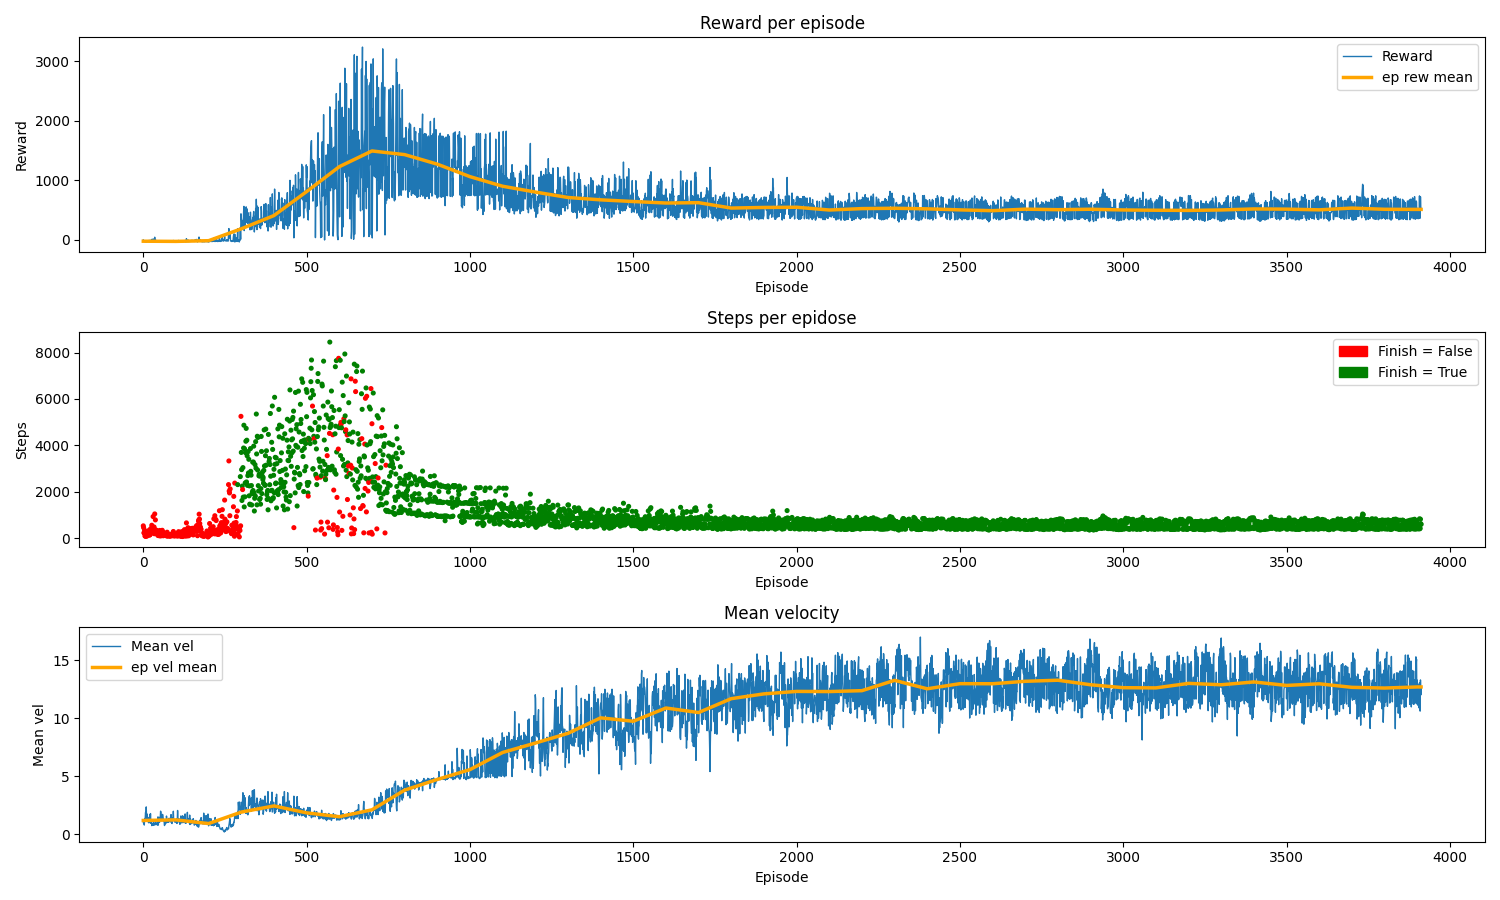
\includegraphics[width=8cm]{figs/Diseño/passing/train_base.png}
  \caption{Datos de entrenamiento sigue-carril para el control adaptativo con \ac{PPO}.}
  \label{fig:passing_train_base}
\end{figure}

\begin{figure}[ht]
  \centering
  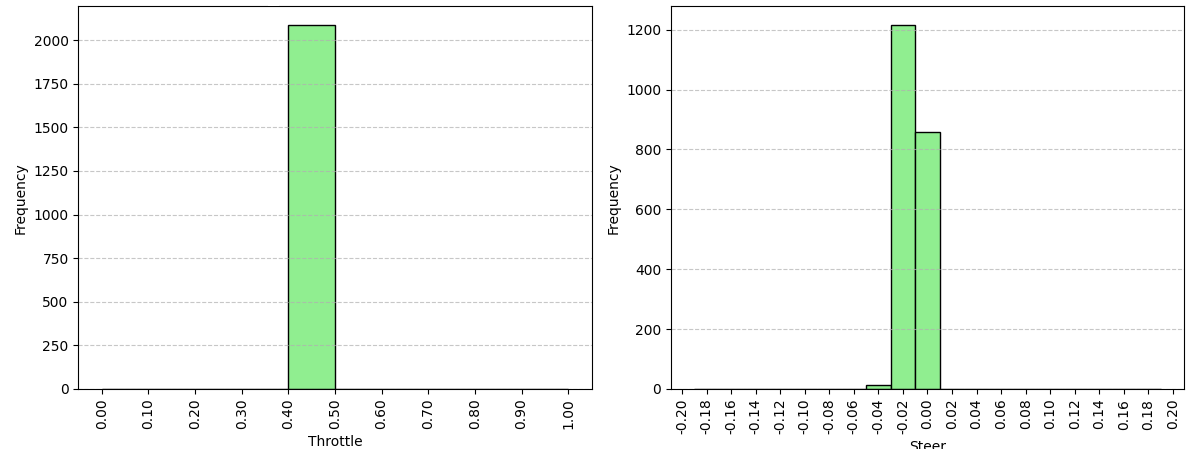
\includegraphics[width=10cm]{figs/Diseño/passing/actions_inference_base.png}
  \caption{Histogramas de acciones tomadas en inferencia durante el sigue-carril para el control adaptativo con \ac{PPO}.}
  \label{fig:passing_actions_inf_base}
\end{figure}

Ahora, necesitamos reentrenar el modelo sigue-carril para lograr un control adaptativo al tráfico. Durante este entrenamiento si activamos la observación del \ac{LiDAR} reales, cuya mínima distancia es incluida y normalizada en la función de recompensa con el fin de conseguir de que el vehículo autónomo sea capaz de circular detrás de un camión adaptándose a su velocidad. Si el coche está a una distancia menor de 4m, se provoca una excepción y se finaliza el episodio dando una recompensa negativa. Se penaliza aún más que salirse del carril, ya que es una acción más grave y que puede tener consecuencias fatales en el mundo real. Los pesos de la función de recompensa cuando vemos el vehículo delantero, dependen de la distancia: cuanto más próximo esté, mayor es la relevancia del \ac{LiDAR}, puesto que aumentan la criticidad de la situación.

\begin{code}[H]
\begin{lstlisting}[language=Python]
if error == None:
    # Deviation normalization, Steer conversion and Throttle conversion

    # LiDAR conversion
    if self._passing and not np.isnan(self._dist_laser):
        r_laser = (np.clip(self._dist_laser, MIN_DIST_LASER, MAX_DIST_LASER) - MIN_DIST_LASER) / (MAX_DIST_LASER - MIN_DIST_LASER)       
    else:
        r_laser = 0

    # Set weights
    # Filter inadequate actions
    elif r_laser != 0:
        if self._dist_laser <= 10:
            w_laser, w_steer, w_dev, w_throttle = 0.9, 0.0, 0.1, 0.0
        elif self._dist_laser <= 12:
            w_laser, w_dev, w_steer, w_throttle = 0.5, 0.45, 0.05, 0.0
        else:
            w_laser, w_dev, w_throttle, w_steer = 0.4, 0.5, 0.05, 0.05
    # Follow lane

    reward = w_dev * r_dev + w_throttle * r_throttle + w_steer * r_steer + w_laser * r_laser
else:
    if "Distance" in error:
        reward = -60
    else:
        reward = -40
\end{lstlisting}
\caption[Función de recompensa respecto al \ac{LiDAR} para control adaptativo con \ac{PPO}]{Función de recompensa respecto al \ac{LiDAR} para control adaptativo con \ac{PPO}.}
\label{cod:rew_ppo_passing}
\end{code}

Como el modelo ya sabe seguir el carril con una velocidad adecuada, no son necesarios tantos episodios de entrenamiento, por lo que hemos reducido el número de \textit{steps} a la mitad, dos millones. También se ha disminuido a la mitad el coeficiente de entropía 0.04, para evitar acciones aleatorias que puedan tener resultados fatales durante el episodio, como provocar una colisión con el camión.

La elección de velocidades del vehículo delantero fue crucial a la hora de lograr un comportamiento estable. Primeramente, se intentó estableciendo una velocidad constante durante un periodo de entre 100 y 450 \textit{steps} en el rango de [5, 10], escogiendo valores enteros y ambos de manera aleatoria. Sin embargo, se encontraron dos problemas:
  \begin{itemize}
        \item Para velocidades altas, el vehículo delantero se alejaba demasiado, sin que el agente pudiera verlo en ningún momento.
        \item El modelo se sobreajustaba a las velocidades bajas, limitándose a alcanzar velocidades máximas de 7 m/s.
    \end{itemize}
Para evitar el primer desafío, se diseñó un compartimento para que el camión delantero se parase si no estaba siendo visto por el agente, pero, aun así, el modelo resultante seguía siendo demasiado lento. Por ello, se modificó este comportamiento para que el camión solo se parase a distancias superiores 30 metros, con la diferencia de distancia entre ambos vehículos se obtuvo directamente del simulador CARLA. De esta forma, garantizamos que el modelo pueda ver al vehículo delantero en todas las velocidades, a la vez que se generen ocasiones en las que no lo vea, lo que ayuda a evitar el sobreajuste del modelo y a mantener las altas velocidades.

\begin{code}[H]
\begin{lstlisting}[language=Python]
if self._count_random % self._random_steps == 0 and self._count_random != 0:
	self._target_vel =  random.randint(5, 10)
	self._random_steps = random.randint(100, 450)
	self._count_random = 0

if loc_ego.distance(self._front_vehicle.get_location()) > 30:
	self._tm.set_desired_speed(self._front_vehicle, 0)  # km/h
else:
	self._tm.set_desired_speed(self._front_vehicle, self._target_vel * 3.6)
	self._count_random += 1
\end{lstlisting}
\caption[Función de recompensa respecto al \ac{LiDAR} para control adaptativo con \ac{PPO}]{Función de recompensa respecto al \ac{LiDAR} para control adaptativo con \ac{PPO}.}
\label{cod:rew_ppo_passing}
\end{code}

El siguiente histograms muestra el número de \textit{steps} durante los que el agente ha observado las diferentes velocidades, así como aquellos en los que no ha detectado el camión delantero durante el reentrenamiento. La fracción de veces que ha visto el camión muy superior a la que no lo ve, pero debemos recordar que en el entrenamiento base de seguimiento de carril no ha visto un vehículo delante en ninguno de los episodios.
\begin{figure}[ht]
  \centering
  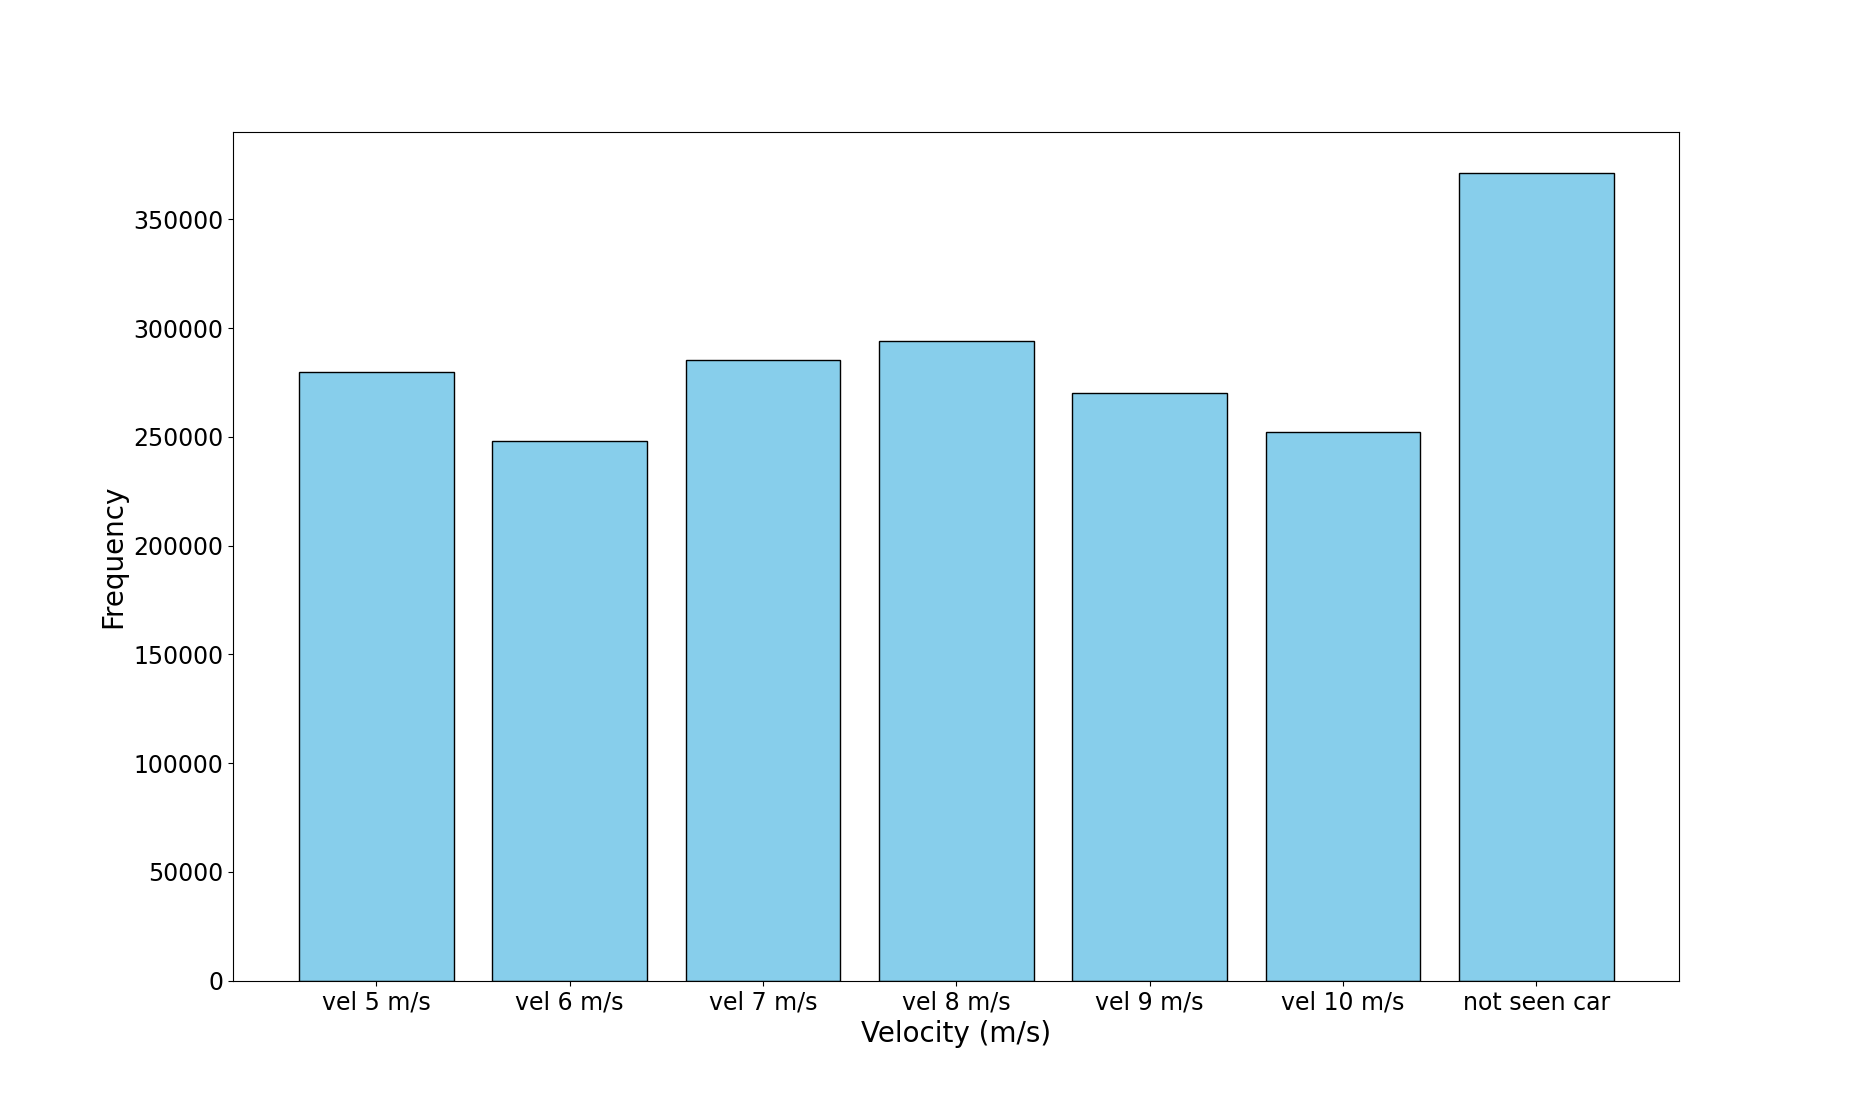
\includegraphics[width=9cm]{figs/Diseño/passing/velocities.png}
  \caption{Histograma de velocidades vistas durante el entrenamiento para el control adaptativo con \ac{PPO}.}
  \label{fig:velocities}
\end{figure}

\newpage

Aunque no se alcanza una convergencia total como en entrenamientos anteriores, podemos decir que el modelo sí converge, ya que la recompensa promedio de los episodios aumenta de manera a lo largo del proceso de entrenamiento. Esto sugiere que, a pesar de los episodios no finalizados, el modelo está mejorando gradualmente su desempeño y aprendiendo de manera efectiva. 
\begin{figure}[ht]
  \centering
  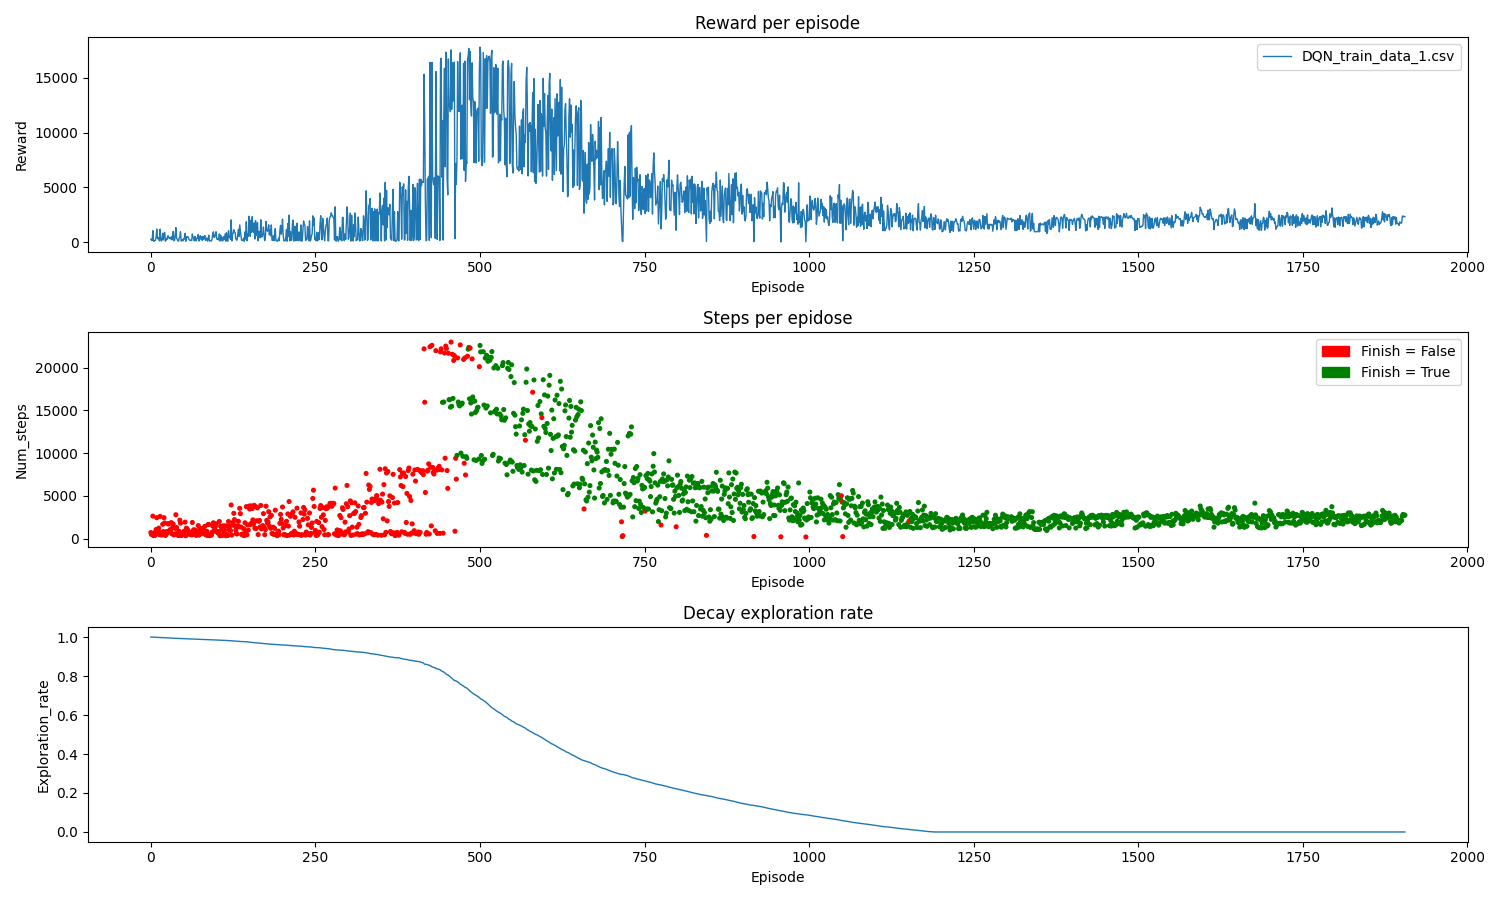
\includegraphics[width=13cm]{figs/Diseño/passing/train.png}
  \caption{Datos de reentrenamiento control adaptativo con \ac{PPO}.}
  \label{fig:velocities}
\end{figure}

En la fase de inferencia, se obtienen buenos resultados a distintas velocidades, tanto altas como bajas, y se sigue manteniendo el seguimiento preciso del carril. La velocidad del coche delantero influye en la distancia de estabilización, es decir, la separación con la que el coche autónomo se mantiene del camión. A mayor velocidad, mayor es esta distancia de seguridad, lo que es lógico y necesario en un entorno real. También se lograr resultados satisfactorios en circuitos no vistos durante el entrenamiento, incluso cambiando de ciudad en CARLA \footnote{\url{https://youtu.be/ieMD1wqqEaY}}. 

Los siguientes diagramas muestran los datos de inferencia recolectados cuando el coche delantero circula a 9 m/s y 5 m/s, respectivamente. Podemos verificar la teoría anterior analizando los histogramas de distancias del \ac{LiDAR}: si el vehículo delantero se desplaza a 9 m/s \footnote{\url{https://youtu.be/mN0Y2q6ny5w}}, el agente mantiene una distancia de unos 14-15 metros; mientras que si circula a 5 m/s \footnote{\url{https://youtu.be/Gvh9ZS0Sizc}}, la distancia se estabiliza en torno a los 13 metros. En cuanto a la velocidad, esta aumenta rápidamente al inicio y luego se estabiliza en un valor cercano al del coche delantero, podemos observar pequeñas fluctuaciones que indican ajustes constantes para mantener la distancia de seguridad. Esto también se refleja en el comportamiento del acelerador, donde la mayoría de las acciones se concentran en el rango [0.4, 0.5], lo que sugiere que el vehículo mantiene una aceleración constante en lugar de realizar ajustes bruscos, logrando así una conducción más suave.

\begin{figure}[ht]
  \centering
  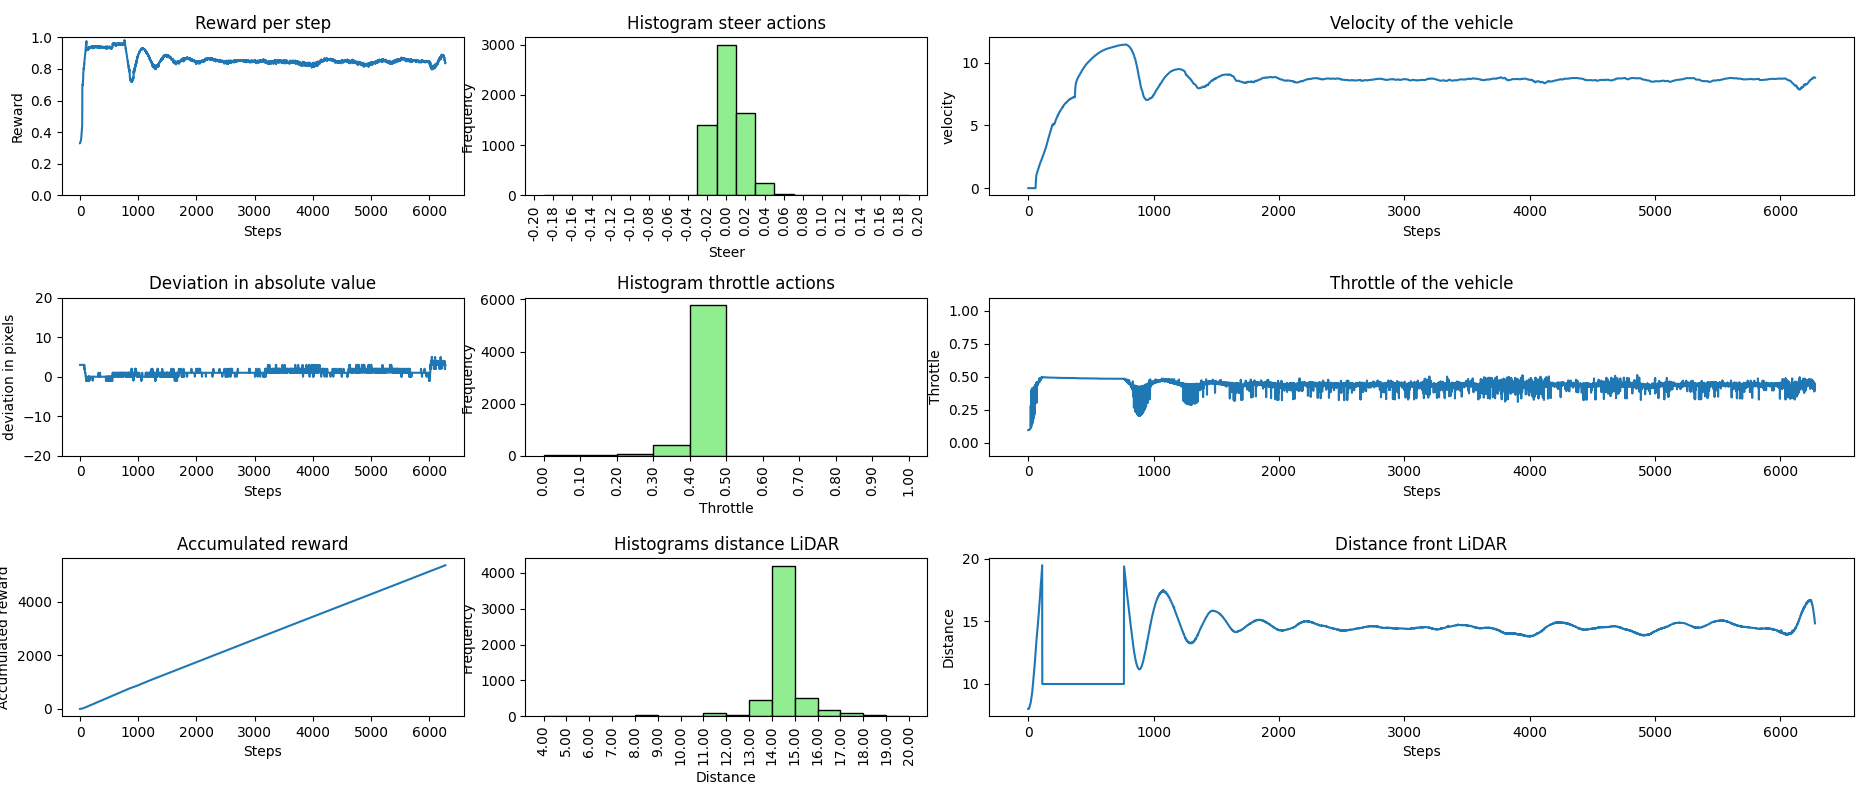
\includegraphics[width=14cm]{figs/Diseño/passing/inference_9.png}
  \caption{Datos de inferencia del control adaptativo con \ac{PPO}, donde el vehículo delantero mantiene una velocidad de 9m/s.}
  \label{fig:infrence_passing}
\end{figure}
\begin{figure}[ht]
  \centering
  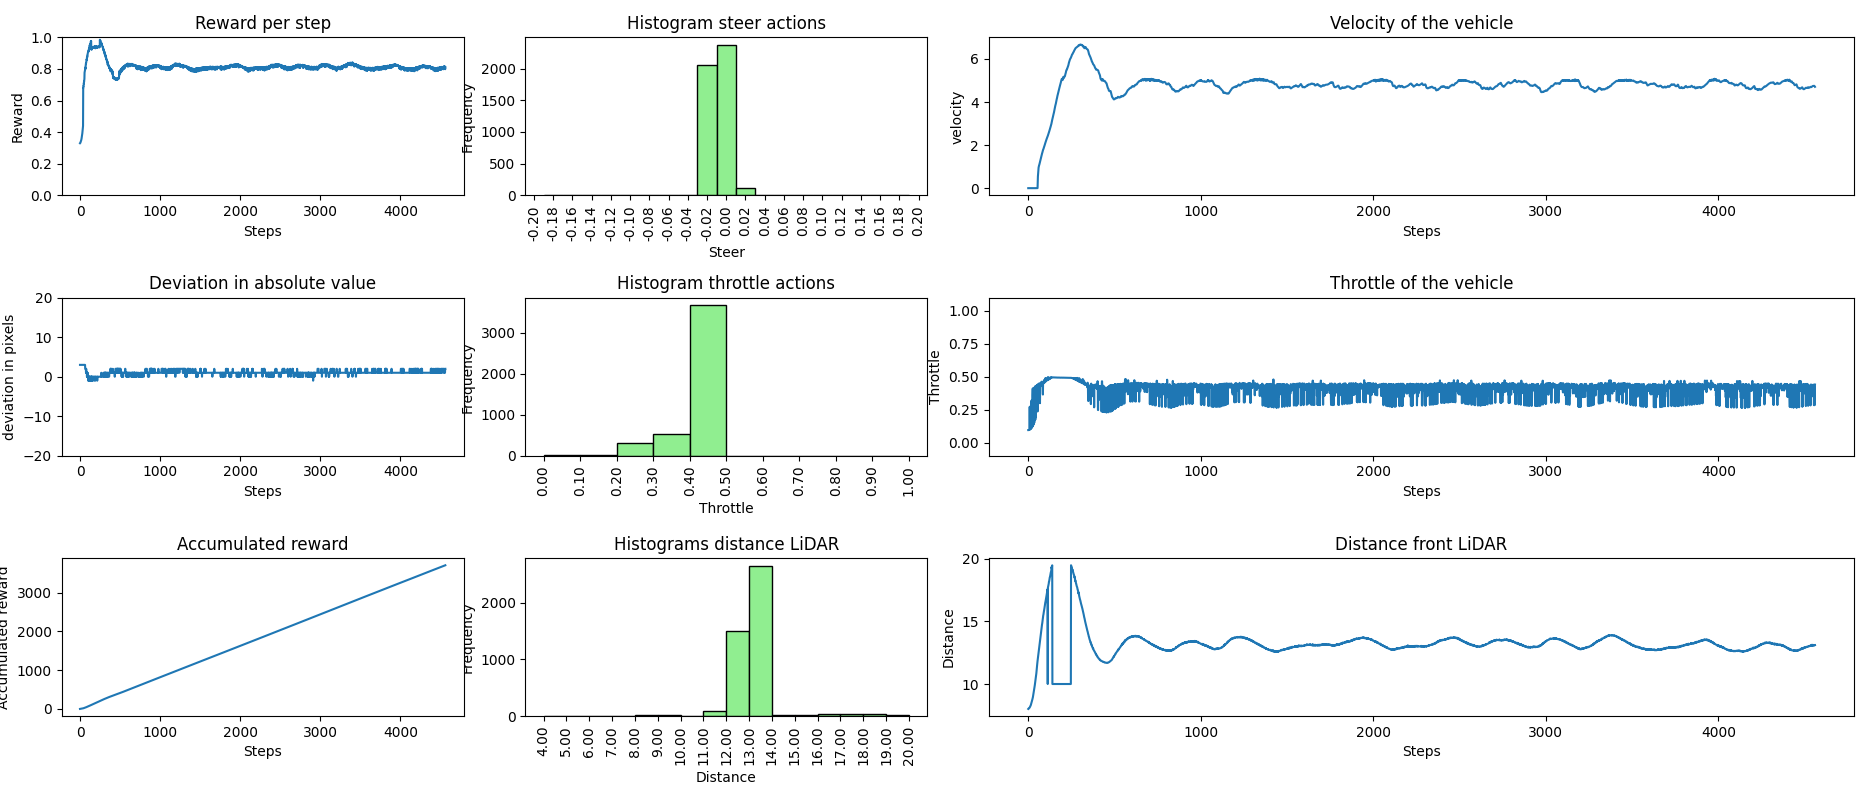
\includegraphics[width=14cm]{figs/Diseño/passing/inference_5.png}
  \caption{Datos de inferencia del control adaptativo con \ac{PPO}, donde el vehículo delantero mantiene una velocidad de 5m/s.}
  \label{fig:infrence_passing}
\end{figure}

\subsection{Maniobra de adelantamiento con PPO}

En este apartado se describe como se ha alcanzo el objetivo final, realizar una maniobra de adelantamiento completa. Cuando se haya visualizado el vehículo delantero a menos de 15 metros, se inicia el cambio de carril a la izquierda y, una vez ya no detectemos el vehículo en la parte derecha del \ac{LiDAR}, el coche autónomo vuelve al carril original. Para ello, es necesario añadir nuevas observaciones al modelo, tanto referentes a la zona derecha del \ac{LiDAR}, como a la segmentación de la calzada. Estas son todas las observaciones que recibe el modelo:
\begin{itemize}
\item Velocidad del propio agente, es decir, del \textit{Ego Vehicle}.
\item Desviación del carril.
\item Centro de masas del carril.
\item Área del carril.
\item 10 puntos de la línea de carril izquierda.
\item 10 puntos de la línea del carril derecha.
\item 10 puntos de la subzona frontal del \ac{LiDAR}.
\item 10 puntos de la subzona frontal derecha del \ac{LiDAR}.
\item 10 puntos de la subzona derecha del \ac{LiDAR}.
\item 10 puntos de la subzona trasera derecha del \ac{LiDAR}.
\item Centro de masas de la calzada.
\item Área de la calzada.
\item 16 puntos del límite izquierdo de la calzada.
\item 16 puntos del límite derecho de la calzada.
\end{itemize}

\begin{figure}[ht]
  \centering
  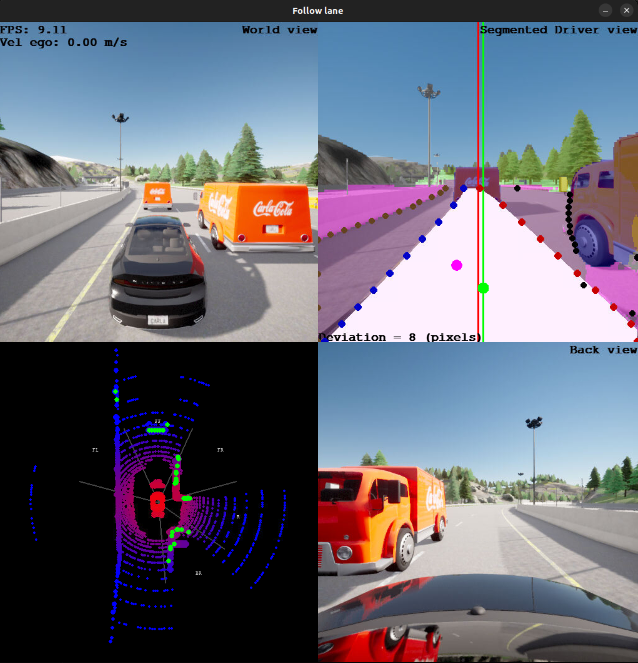
\includegraphics[width=11cm]{figs/Diseño/overtaken/obs.png}
  \caption{Observaciones en el modelo de adelantamiento con \ac{PPO}.}
  \label{fig:obs_overtaken}
\end{figure}

\newpage

Al igual que para el control adaptativo, se realiza un primer entrenamiento para conseguir un modelo capaz de seguir el carril de manera precisa y a altas velocidades. Se ha entrenado a 9 \ac{FPS}, pero esta vez no porque se obtuviera mejoren resultados, sino porque en inferencia se logra ir como máximo a unos 10 \ac{FPS}. Se han reutilizado tanto la función recompensa \ref{cod:rew_carril_ppo_passing} como los hiperparámetros de entrenamiento del modelo sigue-carril para el control adaptativo. Durante este entrenamiento, a diferencia del modelo anterior, no desactivamos las observaciones no relavaste para el seguimiento de carril, el agente recibe constantemente observaciones reales del carril, \ac{LiDAR} y segmentación de la calzada. El circuito usado durante todos entrenamientos, dispone de tres rutas en los que el coche va por el carril más a la derecha en una de ellas y, en las otras dos, por los carriles centrales. Para fomentar la visualización de todos los posibles estados en la calzada, se ha añadido una nueva ruta en la que el vehículo autónomo circula por el carril más a la izquierda, como se puede ver en la Figura \ref{fig:obs_overtaken}. Los resultados han sido…
